\documentclass[aspectratio=169]{beamer}

% =========================================================
% THEME
% =========================================================

\usetheme{metropolis}
\metroset{sectionpage=none}

% =========================================================
% PACKAGES
% =========================================================

\usepackage[french]{babel}
\usepackage[T1]{fontenc}
\usepackage[utf8]{inputenc}
\usepackage{booktabs}
\usepackage{graphicx}
\usepackage{animate}
\usepackage{amsmath}
\usepackage{multirow}
\usepackage{tabularx}
\usepackage{colortbl}
\usepackage{arydshln}
\usepackage[authoryear,round]{natbib}
\usepackage{tikz}
\usetikzlibrary{arrows.meta, positioning, shapes.geometric, calc, fit, backgrounds}
\usepackage{pgfplots}
\usepackage{appendixnumberbeamer}
\usepackage{csquotes}
\usepackage{setspace}

\pgfplotsset{compat=1.18}
\setcitestyle{authoryear,round,aysep={, }}

% =========================================================
% COLORS
% =========================================================

\definecolor{SpaceBlue}{RGB}{15,25,45}
\definecolor{SpaceCyan}{RGB}{0,180,220}
\definecolor{SoftGreen}{RGB}{228,244,235}
\definecolor{SoftOrange}{RGB}{255,242,225}
\definecolor{SoftBlue}{RGB}{230,240,255}
\definecolor{SoftRed}{RGB}{255,232,232}
\definecolor{RuleGreen}{RGB}{126,211,33}
\definecolor{NeuralOrange}{RGB}{245,166,35}

\setbeamercolor{frametitle}{bg=SpaceBlue, fg=white}
\setbeamercolor{title separator}{fg=SpaceCyan}
\setbeamercolor{progress bar}{fg=SpaceCyan}
\setbeamercolor{alerted text}{fg=SpaceBlue}
\hypersetup{
    colorlinks=true,
    citecolor=SpaceBlue,
    linkcolor=SpaceBlue,
    urlcolor=SpaceBlue
}

\setbeamertemplate{itemize item}{\textbullet}
\setbeamertemplate{itemize subitem}{--}
\setbeamertemplate{caption}{\raggedright\insertcaption\par}

% =========================================================
% COMMANDS
% =========================================================

\newcommand{\probP}{\text{I\kern-0.15em P}}
\newcommand{\scite}[1]{{\normalfont\color{SpaceCyan!60!black}[\citealp{#1}]}}
\newcommand{\GridCell}[1]{\node[minimum width=0.78cm,minimum height=0.62cm,draw=SpaceBlue!35,fill=#1] {};}
\newcommand{\TimelineBoxWidth}{2.6cm}
\newcommand{\TimelineBoxHeight}{0.95cm}
\newcommand{\WorldModelWorkshopRef}{%
  \vfill
  {\centering
  \raisebox{-0.18cm}{
\includegraphics[height=0.55cm]{figures/wm_workshop_video.png}}%
  \hspace{0.12cm}%
  \parbox[c]{0.74\textwidth}{%
    \tiny\color{SpaceBlue!75!black}
    Mila -- Quebec AI Institute, World Modeling Workshop, Montréal, 4--6 février 2026.
    \url{https://world-model-mila.github.io/}}%
  \par}
  \vspace{-1cm}
}

\newcommand{\SectionTransitionFrame}[1]{%
  \begin{frame}[plain]
    \centering
    \vfill
    {\Huge\bfseries #1\par}
    \vfill
  \end{frame}
}

\newcommand{\WorldModelTimeline}[1]{%
  \resizebox{0.98\textwidth}{!}{%
    \begin{tikzpicture}[
      x=2.45cm,
      y=1cm,
      font=\scriptsize,
      >=stealth,
      timelinebox/.style={rounded corners=1mm,align=center,text width=\TimelineBoxWidth,minimum height=\TimelineBoxHeight},
      past/.style={timelinebox,draw=SpaceBlue,fill=SoftBlue},
      active/.style={timelinebox,draw=SpaceBlue,fill=SoftOrange,very thick},
      future/.style={timelinebox,draw=SpaceBlue!25,fill=SoftBlue!30,text=SpaceBlue!45}
      ]
      \draw[very thick,->,SpaceBlue!60] (0,0) -- (5.35,0);

      \foreach \x in {0,1.4,2.8,4.0,5.2} {
        \draw[SpaceBlue!55] (\x,0.15)--(\x,-0.15);
      }

      \ifnum#1=1
        \node[active] at (0,-0.92) {\textbf{1943--1990}\\Modèles mentaux\\Apprentissage prédictif};
      \else
        \node[past] at (0,-0.92) {\textbf{1943--1990}\\Modèles mentaux\\Apprentissage prédictif};
      \fi

      \ifnum#1<2
        \node[future] at (1.4,-0.92) {\textbf{1990--2017}\\Modèles prédictifs neuronaux\\RL basé modèle};
      \else\ifnum#1=2
        \node[active] at (1.4,-0.92) {\textbf{1990--2017}\\Modèles prédictifs neuronaux\\RL basé modèle};
      \else
        \node[past] at (1.4,-0.92) {\textbf{1990--2017}\\Modèles prédictifs neuronaux\\RL basé modèle};
      \fi\fi

      \ifnum#1<3
        \node[future] at (2.8,-0.92) {\textbf{2018}\\World Models modernes\\Imagination latente};
      \else\ifnum#1=3
        \node[active] at (2.8,-0.92) {\textbf{2018}\\World Models modernes\\Imagination latente};
      \else
        \node[past] at (2.8,-0.92) {\textbf{2018}\\World Models modernes\\Imagination latente};
      \fi\fi

      \ifnum#1<4
        \node[future] at (4.0,-0.92) {\textbf{2019--2022}\\World Models latents\\Planification latente};
      \else\ifnum#1=4
        \node[active] at (4.0,-0.92) {\textbf{2019--2022}\\World Models latents\\Planification latente};
      \else
        \node[past] at (4.0,-0.92) {\textbf{2019--2022}\\World Models latents\\Planification latente};
      \fi\fi

      \ifnum#1<5
        \node[future] at (5.2,-0.92) {\textbf{2023--Aujourd'hui}\\Foundation World Models\\Vidéo et IA incarnée};
      \else
        \node[active] at (5.2,-0.92) {\textbf{2023--Aujourd'hui}\\Foundation World Models\\Vidéo et IA incarnée};
      \fi
    \end{tikzpicture}
  }%
}

\newcommand{\GridcraftStep}[4]{%
  \begin{tikzpicture}[scale=0.72, every node/.style={font=\scriptsize}]
    \foreach \x in {0,...,4} {
      \foreach \y in {0,...,3} {
        \draw[SpaceBlue!25] (\x,\y) rectangle +(1,1);
      }
    }
    \fill[SpaceBlue!75] (2,1) rectangle +(1,1);
    \fill[RuleGreen!70] #1 rectangle +(1,1);
    \fill[NeuralOrange!80] #2 circle (0.24);
    \node[white,font=\bfseries\scriptsize] at ($#1+(0.5,0.5)$) {A};
    \node[font=\bfseries\scriptsize] at #2 {O};
    \draw[-{Latex[length=2mm]},thick,SpaceCyan] #3;
    \node[align=center,font=\scriptsize] at (2.5,-0.45) {#4};
  \end{tikzpicture}
}

% =========================================================
% TITLE
% =========================================================

\title{
Un Cadre Neuro-Symbolique \\
pour les Modèles du Monde Multi-Agents
}

\author{\textbf{Julien Soulé}$^1$ \and Jean-Paul Jamont$^2$}

\institute{
$^1$SEDAN Research Group -- SnT, University of Luxembourg \\
$^2$Univ. Grenoble Alpes, Grenoble INP, LCIS
}

\logo{
    
\includegraphics[width=0.14\textwidth]{../MASSpace_2026/figures/snt_logo.jpg}
    \hspace{0.35cm}
    
\includegraphics[width=0.065\textwidth]{figures/uga_logo.jpg}
}

\date{
Présentation JFSMA 2026 \\
}

% =========================================================
% BEGIN DOCUMENT
% =========================================================

\begin{document}

{
\setbeamertemplate{footline}{}
\begin{frame}[plain]
  \vspace{0.35cm}
  {\Large\bfseries Un Cadre Neuro-Symbolique\\[0.08cm]
    pour les Modèles du Monde Multi-Agents\par}

  \vspace{0.25cm}
  {\color{SpaceCyan}\rule{0.64\textwidth}{0.8pt}}

  \vspace{0.7cm}
  {\normalsize\textbf{Julien Soulé}$^1$ \hspace{0.4cm} Jean-Paul Jamont$^2$\par}

  \vspace{0.45cm}
  {\scriptsize
    $^1$SEDAN Research Group -- SnT, University of Luxembourg\\
    $^2$Univ. Grenoble Alpes, Grenoble INP, LCIS\par}

  \vfill
  {\scriptsize Présentation JFSMA 2026\par}

  \vspace{0.25cm}
  \begin{flushright}
    
\includegraphics[width=0.13\textwidth]{../MASSpace_2026/figures/snt_logo.jpg}
    \hspace{0.3cm}
    
\includegraphics[width=0.06\textwidth]{figures/uga_logo.jpg}
  \end{flushright}
\end{frame}
}

\setcounter{framenumber}{0}
\logo{}

\section{Contexte}

% \SectionTransitionFrame{Contexte}

\begin{frame}{Les Modèles du Monde : modèles mentaux}
  \scriptsize
  \centering
  \WorldModelTimeline{1}

  \vspace{0.35cm}
  \begin{columns}[T,totalwidth=\textwidth]
    \begin{column}{0.48\textwidth}
      \begin{itemize}
        \setlength{\itemsep}{0.25em}
        \item Un agent peut agir à partir d'une représentation interne du monde.
        \item Cette représentation sert à anticiper les conséquences d'une action.
        \item La prédiction devient déjà une ressource pour le contrôle.
      \end{itemize}
      \vspace{0.05cm}
      \tiny \scite{craik1943,sutton1988}.
    \end{column}
    \begin{column}{0.48\textwidth}
      \[
        s_{t+1}=f(s_t,a_t)
      \]
      \vspace{-0.1cm}
      \begin{itemize}
        \setlength{\itemsep}{0.25em}
        \item $s_t$ : état courant ;
        \item $a_t$ : action choisie ;
        \item $f$ : dynamique supposée connue ou approximée.
      \end{itemize}
    \end{column}
  \end{columns}
  \WorldModelWorkshopRef
\end{frame}

\begin{frame}{Les Modèles du Monde : modèles prédictifs appris}
  \scriptsize
  \centering
  \WorldModelTimeline{2}

  \vspace{0.35cm}
  \begin{columns}[T,totalwidth=\textwidth]
    \begin{column}{0.48\textwidth}
      \begin{itemize}
        \setlength{\itemsep}{0.25em}
        \item La dynamique n'est plus seulement écrite à la main.
        \item Un modèle $\hat{T}_{\phi}$ est appris à partir de transitions (RNN).
        \item Il peut alimenter la planification ou des mises à jour simulées.
      \end{itemize}
      \vspace{0.05cm}
      \tiny \scite{schmidhuber1990,sutton1991,silver2017predictron}.
    \end{column}
    \begin{column}{0.48\textwidth}
      \[
        \hat{T}_{\phi}(s' \mid s,a),
        \qquad
        \hat{R}_{\phi}(s,a)
      \]
      \vspace{-0.1cm}
      \setlength{\itemsep}{0.2em}
      \resizebox{\linewidth}{!}{%
        \begin{tikzpicture}[
          node distance=0.85cm and 1.05cm,
          every node/.style={font=\scriptsize},
          box/.style={draw=SpaceBlue,rounded corners=1mm,align=center,minimum width=2.0cm,minimum height=0.72cm},
          realarr/.style={-{Latex[length=2mm]},thick,SpaceBlue},
          dashedarr/.style={-{Latex[length=2mm]},thick,dashed,NeuralOrange!90!black}
          ]
          \node[box,fill=SoftBlue] (obs) {Etat\\$s_t$};
          \node[box,fill=SoftOrange,right=of obs] (pol) {Politique\\$\pi(a_t|s_t)$};
          \node[box,fill=SoftOrange,right=of pol] (act) {Action\\$a_t$};
          \node[box,fill=SoftGreen,right=of act] (env) {Environnement réel\\$T$};
          \node[box,fill=SoftBlue,below=3.05cm of env] (next) {Nouvel état\\$s_{t+1}$};

          \node[box,fill=white,below=1.05cm of act] (wm) {World model\\$\hat{T}_{\theta}$};
          \node[box,fill=white,below=1.05cm of pol] (pred) {Futur imaginé\\$\hat{s}_{t+1}$};
          \node[box,fill=white,below=1.05cm of obs] (plan) {Planification\\évaluation};

          \draw[realarr] (obs) -- (pol);
          \draw[realarr] (pol) -- (act);
          \draw[realarr] (act) -- (env);
          \draw[realarr] (env) -- (next);
          \draw[realarr] (next.west) -| ([xshift=-0.35cm]obs.west) -- (obs.west);

          \draw[dashedarr] (obs.south) -- (plan.north);
          \draw[dashedarr] (act.south) -- (wm.north);
          \draw[dashedarr] (wm) -- (pred);
          \draw[dashedarr] (pred) -- (plan);
          \draw[dashedarr] (plan.north east) to[bend right=18] node[above,sloped,font=\tiny] {améliore} (pol.south west);

          \node[font=\tiny,align=center,SpaceBlue] at (7.6,0.6) {interactions\\ réelles};
          \node[font=\tiny,align=center,NeuralOrange!90!black] at (4.95,-2.8) {rollouts imaginés};
        \end{tikzpicture}
      }

    \end{column}
  \end{columns}
  \WorldModelWorkshopRef
\end{frame}

\begin{frame}{Les Modèles du Monde : imagination latente}
  \scriptsize
  \centering
  \WorldModelTimeline{3}

  \vspace{0.35cm}
  \begin{columns}[T,totalwidth=\textwidth]
    \begin{column}{0.48\textwidth}
      \textbf{World Models modernes}
      \begin{itemize}
        \setlength{\itemsep}{0.25em}
        \item L'observation est comprimée dans un état latent.
        \item La dynamique est apprise dans cet espace plus compact.
        \item La politique peut être entraînée sur des futurs imaginés.
      \end{itemize}
      \vspace{0.05cm}
      \tiny \scite{ha2018worldmodels}.
    \end{column}
    \begin{column}{0.48\textwidth}
      \vspace{-0.5cm}
      \[
        \begin{aligned}
          z_t                & = Enc(\omega_t),
                             &
          \tilde{h}_t        & = F_{\theta}(\tilde{h}_{t-1},z_t,a_t), \\
          z_{t+1}            & = G_{\theta}(\tilde{h}_t),
                             &
          \hat{r}_{t+1}      & = R_{\theta}(\tilde{h}_t),             \\
          \hat{\omega}_{t+1} & = Dec(z_{t+1})
        \end{aligned}
      \]

      \resizebox{0.84\textwidth}{!}{%
        \begin{tikzpicture}[
          every node/.style={font=\scriptsize},
          box/.style={draw=SpaceBlue,rounded corners=1mm,align=center,minimum width=1.32cm,minimum height=0.68cm},
          arr/.style={-{Latex[length=2mm]},thick,SpaceCyan}
          ]
          \node[box,fill=SoftBlue] (o) at (0,0.25) {$\omega_t$};
          \node[box,fill=SoftBlue] (a) at (0,-1.05) {$a_t$};
          \node[box,fill=white] (hprev) at (0,1.55) {$\tilde{h}_{t-1}$};
          \node[box,fill=SoftGreen] (enc) at (2.15,0.25) {$Enc$\\$z_t$};
          \node[box,fill=SoftOrange] (lstm) at (4.25,0.25) {$F_\theta$\\LSTM};
          \node[box,fill=SoftOrange] (g) at (6.35,0.25) {$G_\theta$\\MLP};
          \node[box,fill=SoftOrange] (r) at (6.35,1.5) {$R_\theta$\\MLP};
          \node[box,fill=SoftBlue] (rout) at (8.45,1.5) {$\hat{r}_{t+1}$};
          \node[box,fill=white] (dec) at (8.45,0.25) {$Dec$};
          \node[box,fill=SoftBlue] (out) at (10.85,0.25) {$\hat{\omega}_{t+1}$};

          \draw[arr] (o) -- (enc);
          \draw[arr] (enc) -- (lstm);
          \draw[arr] (hprev.east) -| (lstm.north);
          \draw[arr] (a.east) -| (lstm.south);
          \draw[arr] (lstm) -- node[above,pos=0.5,yshift=2pt,font=\tiny,text=black] {$\tilde{h}_t$} (g);
          \draw[arr] (lstm.north east) |- node[above,pos=0.55,xshift=7pt,yshift=3pt,font=\tiny,text=black] {$\tilde{h}_t$} (r.west);
          \draw[arr] (r) -- (rout);
          \draw[arr] (g) -- (dec);
          \draw[arr] (dec) -- (out);
        \end{tikzpicture}
      }

    \end{column}
  \end{columns}
  \WorldModelWorkshopRef
\end{frame}

\begin{frame}{Les Modèles du Monde : planification latente}
  \scriptsize
  \centering
  \WorldModelTimeline{4}

  \vspace{0.35cm}
  \begin{columns}[T,totalwidth=\textwidth]
    \begin{column}{0.48\textwidth}
      \textbf{PlaNet, Dreamer}
      \begin{itemize}
        \setlength{\itemsep}{0.25em}
        \item La prédiction devient multi-pas et latente.
        \item Le modèle sert à évaluer des séquences d'actions.
        \item La politique est entraînée dans l'espace latent.
        \item Les erreurs de rollout deviennent centrales.
      \end{itemize}
      \vspace{0.05cm}
      \tiny PlaNet~\scite{hafner2019planet}, Dreamer~\scite{hafner2020dream}.
    \end{column}
    \begin{column}{0.48\textwidth}
      \textbf{Objectif de contrôle}
      \[
        \pi^* =
        \arg\max_{\pi}
        \mathbb{E}_{\hat{T}_{\theta},\pi}
        \left[
          \sum_{k=0}^{H}\gamma^k \hat{r}_{t+k}
          \right]
      \]
    \end{column}
  \end{columns}
  \WorldModelWorkshopRef
\end{frame}

\begin{frame}{Les Modèles du Monde : modèles génériques}
  \scriptsize
  \centering
  \WorldModelTimeline{5}

  \vspace{0.30cm}
  \begin{columns}[T,totalwidth=\textwidth]
    \begin{column}{0.48\textwidth}
      \textbf{Tendance récente}
      \begin{itemize}
        \setlength{\itemsep}{0.25em}
        \item Modèles plus généraux, souvent appris sur vidéo ou environnements variés.
        \item Accent sur l'IA incarnée, la génération et l'adaptation.
        \item Le problème de cohérence reste crucial pour agir dans ces mondes.
      \end{itemize}
      \vspace{0.05cm}
      \tiny DreamerV3~\scite{hafner2023dreamerv3}, Genie~\scite{bruce2024genie},
      V-JEPA~\scite{assran2023vjepa}.
    \end{column}
    \begin{column}{0.48\textwidth}
      \vspace{1.3cm}
      \centering
      \textbf{Quid du Multi-Agent ?}
    \end{column}
  \end{columns}
  \WorldModelWorkshopRef
\end{frame}

\begin{frame}{Difficultés en multi-agent : l'exemple de Gridcraft}
  \begin{columns}[c,totalwidth=\textwidth]
    \begin{column}{0.48\textwidth}
      \scriptsize
      \textbf{Dans un environnement multi-agent partiellement observable}
      \begin{itemize}
        \item les observations locales sont ambiguës \scite{Oliehoek2016} ;
        \item les interactions rendent la dynamique non stationnaire \scite{Wong2023,nekoei2023dealing} ;
        \item les erreurs sont réinjectées dans les rollouts ouverts \scite{talvitie2014modelbias} ;
        \item le mécanisme de transition de l'environnement est implicite \scite{kipf2020contrastivelearningstructuredworld}.
      \end{itemize}
      \textbf{Conséquence: dérive sémantique}
      \begin{itemize}
        \item l'erreur n'est plus seulement numérique,
              elle viole la structure du monde \scite{kipf2020contrastivelearningstructuredworld,talvitie2014modelbias}.
        \item une politique peut planifier dans un monde impossible.
      \end{itemize}
      \vspace{-1cm}
    \end{column}
    \begin{column}{0.49\textwidth}
      \centering
      \animategraphics[
        autoplay,
        loop,
        width=\linewidth
      ]{8}{figures/gridcraft/frame}{0}{37}
      \centering
      \tiny
      Gridcraft est un environnement proposé où trois agents coopèrent dans une grille avec terrain varié (eau, forêts, pierre, chemins) et parcourent une hiérarchie de tâches (collecte, craft, équipement) et luttent contre des zombies mobiles.
    \end{column}
  \end{columns}
\end{frame}

\begin{frame}[shrink=25]{Vers des modèles du monde multi-agents cohérents}

  \scriptsize
  \renewcommand{\arraystretch}{1.2}

  \centering
  \begin{tabular}{p{7.5cm}|p{7.5cm}|p{7.5cm}}
    \toprule
    \textbf{Famille de travaux} &
    \textbf{Contribution}       &
    \textbf{Limites}              \\
    \midrule

    \textbf{World Models neuronaux}

    (World Models, PlaNet, Dreamer)

    \scite{ha2018worldmodels,hafner2020dream}

                                &
    \checkmark\ Dynamique latente apprise

    \checkmark\ Planification par imagination

    \checkmark\ Bonne efficacité en données

                                &
    {\color{red}$\times$} Contraintes du monde uniquement apprises

      {\color{red}$\times$} Accumulation des erreurs lors des rollouts

    \\
    \midrule

    \textbf{Foundation World Models}

    (DreamerV3, Genie, V-JEPA)

    \scite{hafner2023dreamerv3,bruce2024genie,assran2023vjepa}

                                &
    \checkmark\ Généralisation grâce au pré-entraînement massif

    \checkmark\ Capacités émergentes

                                &
    {\color{red}$\times$} Dépend fortement des données et du calcul

      {\color{red}$\times$} Difficilement reproductible dans un contexte académique

    {\color{red}$\times$} Peu de garanties explicites sur les transitions

    \\
    \midrule

    \textbf{World Models multi-agents}

    (MAMBPO, MABL, WM as Graph)

    \scite{wang2020mambpo,wang2022mabl,kipf2020structured}

                                &
    \checkmark\ Modélisation des interactions

    \checkmark\ Représentations plus structurées

                                &
    {\color{red}$\times$} Les contraintes physiques ou logiques restent implicites

      {\color{red}$\times$} La dérive sémantique demeure possible

    \\
    \midrule

    \textbf{World Models neuro-symboliques}

    \scite{agravante2023conversational,balloch2023nswm}

                                &
    \checkmark\ Injection de connaissances métier

    \checkmark\ Contraintes explicites

    \checkmark\ Meilleure interprétabilité

                                &
    {\color{orange}$\triangle$} Travaux principalement en single-agent

    {\color{orange}$\triangle$} Peu d'applications aux WMs multi-agents

    \\
    \midrule
    \midrule

    \rowcolor{blue!7}

    \textbf{Notre positionnement : lorsque certaines \textquote{lois du monde} sont connues, les injecter comme biais inductifs neuro-symboliques dans les WMs multi-agents en complément de la montée en échelle}

                                &
    \checkmark\ Réduire la dérive sémantique moyen-terme en multi-agent et apprentissage en aval.

    \checkmark\ Coût d'entraînement compatible avec la recherche académique.

    \checkmark\ Garanties explicites sur certaines mécaniques de transition.

                                &
    {\color{orange}$\triangle$} Nécessite une connaissance préalable du domaine

      {\color{orange}$\triangle$} Risque d'apprentissage sur-contraint

    {\color{orange}$\triangle$} Ne cherche pas à résoudre tous les problèmes de dérive sémantique

    \\
    \bottomrule
  \end{tabular}

  \vspace{0.15cm}

\end{frame}

% \begin{frame}{Gridcraft : environnement de lecture}
%   \begin{columns}[c,totalwidth=\textwidth]
%     \begin{column}{0.47\textwidth}
%       \scriptsize
%       Gridcraft est volontairement lisible :
%       \begin{itemize}
%         \item trois agents dans une grille partiellement observable ;
%         \item terrain varié : eau, forêts, pierre, chemins irréguliers ;
%         \item hiérarchie de tâches : collecte, craft, équipement, combat ;
%         \item zombies mobiles, fuite avant équipement, chasse ensuite.
%       \end{itemize}

%       \vspace{0.25cm}
%       \textbf{Pourquoi c'est utile ici}
%       \begin{itemize}
%         \item les règles de mouvement et collision sont visibles ;
%         \item les transitions déterminables sont faciles à inspecter ;
%         \item la séparation $\omega^d/\omega^u$ devient concrète.
%       \end{itemize}
%     \end{column}
%     \begin{column}{0.49\textwidth}
%       \centering
%       \animategraphics[
%         autoplay,
%         loop,
%         width=\linewidth
%       ]{8}{figures/gridcraft_overview/gridcraft_overview_}{000}{067}
%     \end{column}
%   \end{columns}
% \end{frame}


\section{Bases}

\SectionTransitionFrame{Bases}

\begin{frame}{Bases : décision partiellement observable}
  \scriptsize
  \begin{columns}[c,totalwidth=\textwidth]
    \begin{column}{0.48\textwidth}
      \textbf{Processus décisionnel de Markov décentralisé partiellement observable}

      \vspace{0.05cm}
      (Decentralized Partially Observable Markov Decision Process -- Dec-POMDP)
      \scite{Oliehoek2016}
      \[
        d=\langle S,\{A_i\}_{i=1}^{n},T,R,\{\Omega_i\}_{i=1}^{n},O,\gamma\rangle
      \]
      \begin{itemize}
        \item chaque agent observe localement $\omega_i \in \Omega_i$ ;
        \item les actions sont conjointes $a^j=(a_1,\ldots,a_n)$ ;
        \item l'objectif est partagé via $R$.
      \end{itemize}
    \end{column}
    \begin{column}{0.48\textwidth}
      \textbf{Apprentissage basé modèle} \scite{Moerland2023modelbased,Wang2022modelbasedmultiagentreinforcementlearning}
      \[
        \hat{T}_{\phi}(s' \mid s,a_1,\ldots,a_n),
        \quad
        \hat{R}_{\phi}(s,a_1,\ldots,a_n)
      \]
      \[
        \hat{O}_{\phi}(\omega' \mid \omega,a_1,\ldots,a_n)
      \]
      \begin{itemize}
        \item apprendre une dynamique approchée ;
        \item simuler des transitions sans interagir avec le monde réel ;
        \item améliorer frugalité en données et planification.
      \end{itemize}
    \end{column}
  \end{columns}
\end{frame}



\begin{frame}{Un modèle du monde multi-agent}
  \scriptsize
  \setlength{\abovedisplayskip}{2pt}
  \setlength{\belowdisplayskip}{2pt}
  \setlength{\abovedisplayshortskip}{2pt}
  \setlength{\belowdisplayshortskip}{2pt}

  Adaptation du modèle de \cite{ha2018worldmodels} avec observation conjointe et action conjointe.

  \begin{columns}[T,totalwidth=\textwidth]
    \begin{column}{0.38\textwidth}
      \[
        \mathcal{T}_{\theta}^j : \mathcal{H} \times \Omega^j \times A^j \rightarrow \Omega^j
      \]
    \end{column}
    \begin{column}{0.60\textwidth}
      \[
        z_t = Enc^j(\mathrm{flatten}(\omega_t^j)), \qquad
        \tilde{h}_t = F_\theta(\tilde{h}_{t-1},z_t,\mathrm{flatten}(a_t^j)), \qquad
      \]
      \[
        \hat{\omega}_{t+1}^j = \mathrm{unflatten}(Dec^j(G_\theta(\tilde{h}_t))), \qquad
        \hat{r}_{t+1}^j = \mathrm{unflatten}(Dec^j(R_\theta(\tilde{h}_t)))
      \]
    \end{column}
  \end{columns}

  \vspace{0.4cm}
  \centering
  \resizebox{0.84\textwidth}{!}{%
    \begin{tikzpicture}[
      every node/.style={font=\scriptsize},
      box/.style={draw=SpaceBlue,rounded corners=1mm,align=center,minimum width=1.32cm,minimum height=0.68cm},
      arr/.style={-{Latex[length=2mm]},thick,SpaceCyan}
      ]
      \node[box,fill=SoftBlue] (o) at (0,0.25) {$\omega_t^j$};
      \node[box,fill=SoftBlue] (a) at (0,-1.05) {$a_t^j$};
      \node[box,fill=white] (hprev) at (0,1.55) {$\tilde{h}_{t-1}$};
      \node[box,fill=SoftGreen] (enc) at (2.15,0.25) {$Enc^j$\\$z_t$};
      \node[box,fill=SoftOrange] (lstm) at (4.25,0.25) {$F_\theta$\\LSTM};
      \node[box,fill=SoftOrange] (g) at (6.35,0.25) {$G_\theta$\\MLP};
      \node[box,fill=SoftOrange] (r) at (6.35,1.5) {$R_\theta$\\MLP};
      \node[box,fill=SoftBlue] (rout) at (8.45,1.5) {$\hat{r}_{t+1}$};
      \node[box,fill=white] (dec) at (8.45,0.25) {$Dec^j$};
      \node[box,fill=SoftBlue] (out) at (10.85,0.25) {$\hat{\omega}_{t+1}^j$};

      \draw[arr] (o) -- node[above,pos=0.5,yshift=2pt,font=\tiny] {flatten} (enc);
      \draw[arr] (enc) -- (lstm);
      \draw[arr] (hprev.east) -| (lstm.north);
      \draw[arr] (a.east) -| node[pos=0.28,below,font=\tiny] {flatten} (lstm.south);
      \draw[arr] (lstm) -- node[above,pos=0.5,yshift=2pt,font=\tiny,text=black] {$\tilde{h}_t$} (g);
      \draw[arr] (lstm.north east) |- node[above,pos=0.55,xshift=7pt,yshift=3pt,font=\tiny,text=black] {$\tilde{h}_t$} (r.west);
      \draw[arr] (r) -- (rout);
      \draw[arr] (g) -- (dec);
      \draw[arr] (dec) -- node[above,pos=0.5,yshift=2pt,font=\tiny] {unflatten} (out);
    \end{tikzpicture}
  }

  \vspace{0.4cm}

  \begin{block}{}
    \tiny
    Modèle du monde multi-agent (Multi-Agent World Model -- MAWM)
    pour l'apprentissage par renforcement multi-agent basé modèle
    (Model-Based Multi-Agent Reinforcement Learning -- MB-MARL).
    Le modèle de prédiction d'observation conjointe
    (Joint-Observation Prediction Model -- JOPM) utilise $F_\theta$ comme mémoire
    longue à court terme (Long Short-Term Memory -- LSTM), $G_\theta$ et $R_\theta$ comme
    perceptrons multicouche (Multi-Layer Perceptron -- MLP)
    \scite{ha2018worldmodels,hafner2020dreamer}.
  \end{block}

\end{frame}

\section{Cadre neuro-symbolique}

\SectionTransitionFrame{Cadre neuro-symbolique}

\begin{frame}{Hypothèses de travail}
  \scriptsize

  \vspace{0.12cm}
  \begin{itemize}
    \item Certaines composantes du vecteur d'observation seraient déterminables à partir de règles symboliques assimilables à des \textquote{mécanismes inhérents à l'environnement}.

    \item Le Modèle du Monde neuronal pourrait être guidé par des règles symboliques pour éviter la dérive sémantique.

    \item La prédiction du Modèle du Monde neuronal pourrait être corrigée par des règles symboliques pour éviter la dérive sémantique.

    \item Le Modèle du Monde neuronal gagnerait à se concentrer sa capacité sur ce qui reste
          incertain, plutôt qu'à réapprendre des contraintes déjà connues.

    \item La cohérence du Modèle du Monde avec les règles de transition devrait être mesurée explicitement.
  \end{itemize}
\end{frame}

\begin{frame}{Espace latent d'observation structuré}
  \vspace{0.6cm}
  \scriptsize
  \begin{columns}[c,totalwidth=\textwidth]
    \begin{column}{0.49\textwidth}
      \textbf{Observation structurée}
      \vspace{-0.2cm}
      \[
        \text{Supposons }\omega_{i,t} = concat(\omega^d_{i,t}, \omega^u_{i,t}) = \left(f^d_{1,t}, \ldots, f^d_{m,t}, f^u_{m+1,t}, \ldots, f^u_{n_f,t}\right)
      \]
      \vspace{-0.6cm}
      \begin{itemize}
        \item $\omega^d$ : caractéristiques déterminables par règles ;
        \item $\omega^u$ : caractéristiques indéterminables, apprises par données ;
      \end{itemize}

      On introduit un \textbf{Partial Symbolic World Model} (PSWM) $\mathcal{T}_s^j$ prédisant une \textquote{partie du futur}.

      \vspace{0.1cm}

      \begin{block}{\scriptsize Exemple avec Gridcraft}
        \begin{itemize}
          \item $\omega^d$ : terrain/block statiques connus, agent au centre, autres agents localisés, inventaire/craft déterministe ;
          \item $\omega^u$ : nouvelles cellules inconnues, mobs/zombies, drops aléatoires, événements non observables, effets ambigus ou stochastiques.
        \end{itemize}
      \end{block}

    \end{column}
    \begin{column}{0.45\textwidth}
      \centering
      \resizebox{\linewidth}{!}{%
        \begin{tikzpicture}[
          every node/.style={font=\scriptsize},
          arr/.style={-{Latex[length=2mm]},thick,SpaceCyan}
          ]
          \draw[draw=SpaceBlue,fill=white] (0,0) rectangle (1.0,3.2);
          \fill[NeuralOrange!80] (0,1.6) rectangle (1.0,3.2);
          \fill[RuleGreen!80] (0,0) rectangle (1.0,1.6);
          \node at (0.5,2.4) {$\omega^u$};
          \node at (0.5,0.8) {$\omega^d$};
          \node[align=center] at (0.5,-0.35) {observation\\courante};

          \node[draw=SpaceBlue,rounded corners=1mm,fill=SoftGreen,align=center,minimum width=2.0cm,minimum height=0.8cm] at (3.3,0.8) (symb) {$\mathcal{T}_s^j$\\règles};
          \node[draw=SpaceBlue,rounded corners=1mm,fill=SoftOrange,align=center,minimum width=2.0cm,minimum height=0.8cm] at (3.3,2.4) (neur) {$\mathcal{T}_\theta^j$\\réseau};

          \draw[draw=SpaceBlue,fill=white] (5.6,0) rectangle (6.6,3.2);
          \fill[NeuralOrange!80] (5.6,1.6) rectangle (6.6,3.2);
          \fill[RuleGreen!80] (5.6,0) rectangle (6.6,1.6);
          \node at (6.1,2.4) {$\hat{\omega}^u$};
          \node at (6.1,0.8) {$\hat{\omega}^d$};
          \node[align=center] at (6.1,-0.35) {futur\\hybride};

          \draw[dashed,arr] (1.0,0.8) -- (symb);
          \draw[dashed,arr] (1.0,0.8) -- (neur);
          \draw[dashed,arr] (1.0,2.4) -- (neur);
          \draw[dashed,arr] (symb) -- (5.6,0.8);
          \draw[dashed,arr] (neur) -- (5.6,2.4);
          \draw[dashed,arr] (neur) -- (5.6,0.8);
        \end{tikzpicture}
      }

      \vspace{0.2cm}

      Couverture : $\kappa = \frac{\text{nombre de caractéristiques couvertes par les PSTR}}{\text{nombre total de caractéristiques}}$

      \vspace{-1cm}

    \end{column}

  \end{columns}
\end{frame}

\begin{frame}{Règle de transition symbolique partielle}
  \scriptsize
  On introduit une \textit{Partial Symbolic Transition Rule} (PSTR) décrivant un mécanisme de transition symbolique partielle.
  \[
    s_i(h^j_{t-1}, \omega^j_t, a^j_t) = \{f^d_{l,t+1}, \ldots, f^d_{m,t+1}\}^j = \omega_{i,t+1}^{d,j}
  \]
  \vspace{-0.45cm}
  \begin{columns}[c,totalwidth=\textwidth]
    \begin{column}{0.38\textwidth}
      \begin{itemize}
        \item \textbf{entrée} : observation locale ou conjointe, action, historique ;
        \item \textbf{sortie} : sous-ensemble de caractéristiques déterminables ;
        \item les caractéristiques inconnues restent au réseau neuronal ;
        \item les violations de ces règles devraient être comptabilisées.
      \end{itemize}
    \end{column}
    \begin{column}{0.58\textwidth}
      \centering
      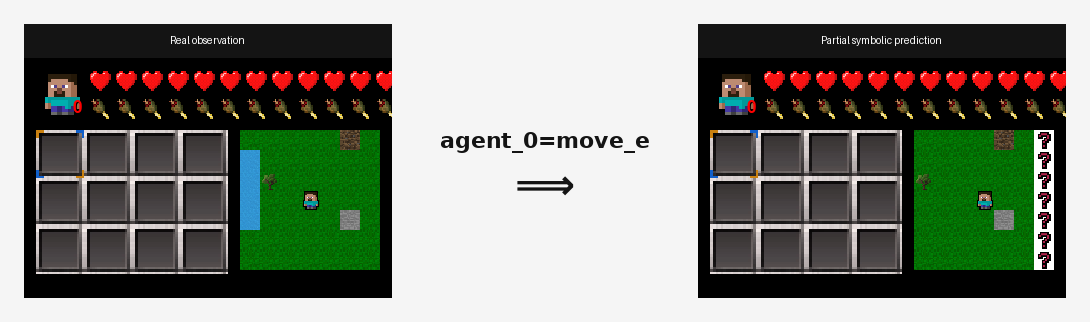
\includegraphics[width=\linewidth]{figures/pstr_viz/PSTR_INDIV_LOCAL_GRID_TRANSLATION.png}

      \vspace{0.08cm}
      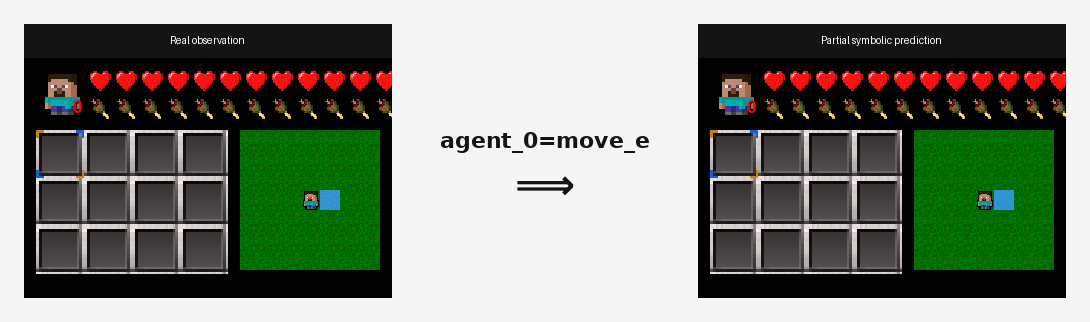
\includegraphics[width=\linewidth]{figures/pstr_viz/PSTR_INDIV_BLOCKED_WATER.png}
    \end{column}
  \end{columns}

  L'agrégation des règles PSTR donne un modèle PSWM : $\mathcal{T}^j_s(h^j_{t-1}, \omega^j_t, a^j_t) = \bigcup_{i \in n_{PSTR}} \omega_{i,t+1}^{d,j} = \omega^{d,j}_{t+1} $

\end{frame}

\begin{frame}{Stratégies d'intégration neuro-symbolique}

  \begin{columns}[c,totalwidth=\textwidth]
    \begin{column}{0.5\textwidth}
      \centering
      \vspace{-1cm}
      \resizebox{!}{0.97\textheight}{


\tikzset{every picture/.style={line width=0.75pt}} %set default line width to 0.75pt        

\begin{tikzpicture}[x=0.75pt,y=0.75pt,yscale=-1,xscale=1]
    %uncomment if require: \path (0,5232); %set diagram left start at 0, and has height of 5232

    %Straight Lines [id:da24763982027429865] 
    \draw [color={rgb, 255:red, 155; green, 155; blue, 155 }  ,draw opacity=1 ][fill={rgb, 255:red, 128; green, 128; blue, 128 }  ,fill opacity=1 ][line width=0.75]    (402,4448) -- (384,4470) ;
    %Straight Lines [id:da19980478632170595] 
    \draw [color={rgb, 255:red, 155; green, 155; blue, 155 }  ,draw opacity=1 ][fill={rgb, 255:red, 128; green, 128; blue, 128 }  ,fill opacity=1 ][line width=0.75]    (396,4448) -- (384,4462) ;
    %Straight Lines [id:da32412855340391855] 
    \draw [color={rgb, 255:red, 155; green, 155; blue, 155 }  ,draw opacity=1 ][fill={rgb, 255:red, 128; green, 128; blue, 128 }  ,fill opacity=1 ][line width=0.75]    (406,4450) -- (390,4470) ;
    %Straight Lines [id:da21125524013600872] 
    \draw [color={rgb, 255:red, 155; green, 155; blue, 155 }  ,draw opacity=1 ][fill={rgb, 255:red, 128; green, 128; blue, 128 }  ,fill opacity=1 ][line width=0.75]    (406,4456) -- (396,4470) ;
    %Straight Lines [id:da8737340062156574] 
    \draw [color={rgb, 255:red, 155; green, 155; blue, 155 }  ,draw opacity=1 ][fill={rgb, 255:red, 128; green, 128; blue, 128 }  ,fill opacity=1 ][line width=0.75]    (406,4464) -- (402,4470) ;
    %Straight Lines [id:da2890333682601931] 
    \draw [color={rgb, 255:red, 155; green, 155; blue, 155 }  ,draw opacity=1 ][fill={rgb, 255:red, 128; green, 128; blue, 128 }  ,fill opacity=1 ][line width=0.75]    (384,4454) -- (390,4448) ;
    %Straight Lines [id:da4621444959459615] 
    \draw [color={rgb, 255:red, 155; green, 155; blue, 155 }  ,draw opacity=1 ][fill={rgb, 255:red, 128; green, 128; blue, 128 }  ,fill opacity=1 ][line width=0.75]    (406,4332) -- (384,4360) ;
    %Straight Lines [id:da5637690900595229] 
    \draw [color={rgb, 255:red, 155; green, 155; blue, 155 }  ,draw opacity=1 ][fill={rgb, 255:red, 128; green, 128; blue, 128 }  ,fill opacity=1 ][line width=0.75]    (400,4332) -- (384,4352) ;
    %Straight Lines [id:da7986277651239229] 
    \draw [color={rgb, 255:red, 155; green, 155; blue, 155 }  ,draw opacity=1 ][fill={rgb, 255:red, 128; green, 128; blue, 128 }  ,fill opacity=1 ][line width=0.75]    (406,4340) -- (390,4360) ;
    %Straight Lines [id:da2888528174156788] 
    \draw [color={rgb, 255:red, 155; green, 155; blue, 155 }  ,draw opacity=1 ][fill={rgb, 255:red, 128; green, 128; blue, 128 }  ,fill opacity=1 ][line width=0.75]    (406,4348) -- (396,4360) ;
    %Straight Lines [id:da21145998471436278] 
    \draw [color={rgb, 255:red, 155; green, 155; blue, 155 }  ,draw opacity=1 ][fill={rgb, 255:red, 128; green, 128; blue, 128 }  ,fill opacity=1 ][line width=0.75]    (406,4356) -- (402,4360) ;
    %Straight Lines [id:da259794037058905] 
    \draw [color={rgb, 255:red, 155; green, 155; blue, 155 }  ,draw opacity=1 ][fill={rgb, 255:red, 128; green, 128; blue, 128 }  ,fill opacity=1 ][line width=0.75]    (384,4344) -- (394,4332) ;
    %Straight Lines [id:da37905992722226245] 
    \draw [color={rgb, 255:red, 155; green, 155; blue, 155 }  ,draw opacity=1 ][fill={rgb, 255:red, 128; green, 128; blue, 128 }  ,fill opacity=1 ][line width=0.75]    (384,4336) -- (388,4332) ;

    %Straight Lines [id:da4618897886186095] 
    \draw [color={rgb, 255:red, 155; green, 155; blue, 155 }  ,draw opacity=1 ][fill={rgb, 255:red, 128; green, 128; blue, 128 }  ,fill opacity=1 ][line width=0.75]    (406,4498) -- (384,4526) ;
    %Straight Lines [id:da9618492285817379] 
    \draw [color={rgb, 255:red, 155; green, 155; blue, 155 }  ,draw opacity=1 ][fill={rgb, 255:red, 128; green, 128; blue, 128 }  ,fill opacity=1 ][line width=0.75]    (400,4498) -- (384,4518) ;
    %Straight Lines [id:da4047027863035557] 
    \draw [color={rgb, 255:red, 155; green, 155; blue, 155 }  ,draw opacity=1 ][fill={rgb, 255:red, 128; green, 128; blue, 128 }  ,fill opacity=1 ][line width=0.75]    (406,4506) -- (390,4526) ;
    %Straight Lines [id:da2338233317691657] 
    \draw [color={rgb, 255:red, 155; green, 155; blue, 155 }  ,draw opacity=1 ][fill={rgb, 255:red, 128; green, 128; blue, 128 }  ,fill opacity=1 ][line width=0.75]    (406,4514) -- (396,4526) ;
    %Straight Lines [id:da040061497129813106] 
    \draw [color={rgb, 255:red, 155; green, 155; blue, 155 }  ,draw opacity=1 ][fill={rgb, 255:red, 128; green, 128; blue, 128 }  ,fill opacity=1 ][line width=0.75]    (406,4522) -- (402,4526) ;
    %Straight Lines [id:da8926300803967907] 
    \draw [color={rgb, 255:red, 155; green, 155; blue, 155 }  ,draw opacity=1 ][fill={rgb, 255:red, 128; green, 128; blue, 128 }  ,fill opacity=1 ][line width=0.75]    (384,4510) -- (394,4498) ;
    %Straight Lines [id:da8033717813225199] 
    \draw [color={rgb, 255:red, 155; green, 155; blue, 155 }  ,draw opacity=1 ][fill={rgb, 255:red, 128; green, 128; blue, 128 }  ,fill opacity=1 ][line width=0.75]    (384,4502) -- (388,4498) ;

    %Straight Lines [id:da7989858669141804] 
    \draw [color={rgb, 255:red, 155; green, 155; blue, 155 }  ,draw opacity=1 ][fill={rgb, 255:red, 128; green, 128; blue, 128 }  ,fill opacity=1 ][line width=0.75]    (408,4659.05) -- (386,4687.05) ;
    %Straight Lines [id:da40202240481802576] 
    \draw [color={rgb, 255:red, 155; green, 155; blue, 155 }  ,draw opacity=1 ][fill={rgb, 255:red, 128; green, 128; blue, 128 }  ,fill opacity=1 ][line width=0.75]    (402,4659.05) -- (386,4679.05) ;
    %Straight Lines [id:da23397697614023283] 
    \draw [color={rgb, 255:red, 155; green, 155; blue, 155 }  ,draw opacity=1 ][fill={rgb, 255:red, 128; green, 128; blue, 128 }  ,fill opacity=1 ][line width=0.75]    (408,4667.05) -- (392,4687.05) ;
    %Straight Lines [id:da5091139872418293] 
    \draw [color={rgb, 255:red, 155; green, 155; blue, 155 }  ,draw opacity=1 ][fill={rgb, 255:red, 128; green, 128; blue, 128 }  ,fill opacity=1 ][line width=0.75]    (408,4675.05) -- (398,4687.05) ;
    %Straight Lines [id:da7838519186238893] 
    \draw [color={rgb, 255:red, 155; green, 155; blue, 155 }  ,draw opacity=1 ][fill={rgb, 255:red, 128; green, 128; blue, 128 }  ,fill opacity=1 ][line width=0.75]    (408,4683.05) -- (404,4687.05) ;
    %Straight Lines [id:da15998290322205744] 
    \draw [color={rgb, 255:red, 155; green, 155; blue, 155 }  ,draw opacity=1 ][fill={rgb, 255:red, 128; green, 128; blue, 128 }  ,fill opacity=1 ][line width=0.75]    (386,4671.05) -- (396,4659.05) ;
    %Straight Lines [id:da2930214299406628] 
    \draw [color={rgb, 255:red, 155; green, 155; blue, 155 }  ,draw opacity=1 ][fill={rgb, 255:red, 128; green, 128; blue, 128 }  ,fill opacity=1 ][line width=0.75]    (386,4663.05) -- (390,4659.05) ;

    %Straight Lines [id:da560381072959208] 
    \draw [color={rgb, 255:red, 155; green, 155; blue, 155 }  ,draw opacity=1 ][fill={rgb, 255:red, 128; green, 128; blue, 128 }  ,fill opacity=1 ][line width=0.75]    (408,4745.05) -- (386,4773.05) ;
    %Straight Lines [id:da019087143657265826] 
    \draw [color={rgb, 255:red, 155; green, 155; blue, 155 }  ,draw opacity=1 ][fill={rgb, 255:red, 128; green, 128; blue, 128 }  ,fill opacity=1 ][line width=0.75]    (402,4745.05) -- (386,4765.05) ;
    %Straight Lines [id:da1302277202981762] 
    \draw [color={rgb, 255:red, 155; green, 155; blue, 155 }  ,draw opacity=1 ][fill={rgb, 255:red, 128; green, 128; blue, 128 }  ,fill opacity=1 ][line width=0.75]    (408,4753.05) -- (392,4773.05) ;
    %Straight Lines [id:da09652292926698536] 
    \draw [color={rgb, 255:red, 155; green, 155; blue, 155 }  ,draw opacity=1 ][fill={rgb, 255:red, 128; green, 128; blue, 128 }  ,fill opacity=1 ][line width=0.75]    (408,4761.05) -- (398,4773.05) ;
    %Straight Lines [id:da7503736353080281] 
    \draw [color={rgb, 255:red, 155; green, 155; blue, 155 }  ,draw opacity=1 ][fill={rgb, 255:red, 128; green, 128; blue, 128 }  ,fill opacity=1 ][line width=0.75]    (408,4769.05) -- (404,4773.05) ;
    %Straight Lines [id:da5657791005138578] 
    \draw [color={rgb, 255:red, 155; green, 155; blue, 155 }  ,draw opacity=1 ][fill={rgb, 255:red, 128; green, 128; blue, 128 }  ,fill opacity=1 ][line width=0.75]    (386,4757.05) -- (396,4745.05) ;
    %Straight Lines [id:da24043326957092126] 
    \draw [color={rgb, 255:red, 155; green, 155; blue, 155 }  ,draw opacity=1 ][fill={rgb, 255:red, 128; green, 128; blue, 128 }  ,fill opacity=1 ][line width=0.75]    (386,4749.05) -- (390,4745.05) ;

    %Shape: Rectangle [id:dp9707159588190506] 
    \draw   (72,4360) -- (202,4360) -- (202,4450) -- (72,4450) -- cycle ;
    %Shape: Rectangle [id:dp5706382238892072] 
    \draw   (328,4328) -- (430,4328) -- (430,4474) -- (328,4474) -- cycle ;
    %Straight Lines [id:da7375663634648962] 
    \draw    (190,4382) -- (250,4382) ;
    \draw [shift={(252,4382)}, rotate = 180] [color={rgb, 255:red, 0; green, 0; blue, 0 }  ][line width=0.75]    (10.93,-3.29) .. controls (6.95,-1.4) and (3.31,-0.3) .. (0,0) .. controls (3.31,0.3) and (6.95,1.4) .. (10.93,3.29)   ;
    %Straight Lines [id:da1312146218906476] 
    \draw    (191.68,4428) -- (246,4428) ;
    \draw [shift={(248,4428)}, rotate = 180] [color={rgb, 255:red, 0; green, 0; blue, 0 }  ][line width=0.75]    (10.93,-3.29) .. controls (6.95,-1.4) and (3.31,-0.3) .. (0,0) .. controls (3.31,0.3) and (6.95,1.4) .. (10.93,3.29)   ;
    %Straight Lines [id:da20293234879784128] 
    \draw    (278,4382) -- (338,4382) ;
    \draw [shift={(340,4382)}, rotate = 180] [color={rgb, 255:red, 0; green, 0; blue, 0 }  ][line width=0.75]    (10.93,-3.29) .. controls (6.95,-1.4) and (3.31,-0.3) .. (0,0) .. controls (3.31,0.3) and (6.95,1.4) .. (10.93,3.29)   ;
    %Straight Lines [id:da7780554830331595] 
    \draw    (284,4428) -- (338,4428) ;
    \draw [shift={(340,4428)}, rotate = 180] [color={rgb, 255:red, 0; green, 0; blue, 0 }  ][line width=0.75]    (10.93,-3.29) .. controls (6.95,-1.4) and (3.31,-0.3) .. (0,0) .. controls (3.31,0.3) and (6.95,1.4) .. (10.93,3.29)   ;
    %Shape: Rectangle [id:dp9989891710916556] 
    \draw   (118,4364) -- (198,4364) -- (198,4446) -- (118,4446) -- cycle ;
    %Shape: Rectangle [id:dp5273520585937012] 
    \draw   (72,4684) -- (202,4684) -- (202,4774) -- (72,4774) -- cycle ;
    %Straight Lines [id:da11653013315343552] 
    \draw    (192,4753.05) -- (222,4753.05) ;
    \draw [shift={(224,4753.05)}, rotate = 180] [color={rgb, 255:red, 0; green, 0; blue, 0 }  ][line width=0.75]    (10.93,-3.29) .. controls (6.95,-1.4) and (3.31,-0.3) .. (0,0) .. controls (3.31,0.3) and (6.95,1.4) .. (10.93,3.29)   ;
    %Straight Lines [id:da2685409551114073] 
    \draw    (250,4712.05) -- (338,4712.05) ;
    \draw [shift={(340,4712.05)}, rotate = 180] [color={rgb, 255:red, 0; green, 0; blue, 0 }  ][line width=0.75]    (10.93,-3.29) .. controls (6.95,-1.4) and (3.31,-0.3) .. (0,0) .. controls (3.31,0.3) and (6.95,1.4) .. (10.93,3.29)   ;
    %Straight Lines [id:da6588342775342261] 
    \draw    (316,4753.05) -- (333.67,4753.05) -- (338,4753.05) ;
    \draw [shift={(340,4753.05)}, rotate = 180] [color={rgb, 255:red, 0; green, 0; blue, 0 }  ][line width=0.75]    (10.93,-3.29) .. controls (6.95,-1.4) and (3.31,-0.3) .. (0,0) .. controls (3.31,0.3) and (6.95,1.4) .. (10.93,3.29)   ;
    %Shape: Rectangle [id:dp9055792744513167] 
    \draw   (118,4688) -- (198,4688) -- (198,4770) -- (118,4770) -- cycle ;
    %Straight Lines [id:da005030131609338517] 
    \draw    (432,4761.05) -- (432,4831.05) -- (236,4831.05) -- (236,4769.05) ;
    \draw [shift={(236,4767.05)}, rotate = 90] [color={rgb, 255:red, 0; green, 0; blue, 0 }  ][line width=0.75]    (10.93,-3.29) .. controls (6.95,-1.4) and (3.31,-0.3) .. (0,0) .. controls (3.31,0.3) and (6.95,1.4) .. (10.93,3.29)   ;
    %Straight Lines [id:da24266384766556137] 
    \draw    (380,4719.05) -- (412,4719.05) ;
    \draw [shift={(414,4719.05)}, rotate = 180] [color={rgb, 255:red, 0; green, 0; blue, 0 }  ][line width=0.75]    (10.93,-3.29) .. controls (6.95,-1.4) and (3.31,-0.3) .. (0,0) .. controls (3.31,0.3) and (6.95,1.4) .. (10.93,3.29)   ;
    %Straight Lines [id:da7310522190261277] 
    \draw    (380,4738) -- (412,4738) ;
    \draw [shift={(414,4738)}, rotate = 180] [color={rgb, 255:red, 0; green, 0; blue, 0 }  ][line width=0.75]    (10.93,-3.29) .. controls (6.95,-1.4) and (3.31,-0.3) .. (0,0) .. controls (3.31,0.3) and (6.95,1.4) .. (10.93,3.29)   ;
    %Shape: Rectangle [id:dp7311570933646381] 
    \draw   (72,4525) -- (202,4525) -- (202,4615) -- (72,4615) -- cycle ;
    %Straight Lines [id:da3798900997456174] 
    \draw    (190,4547) -- (250,4547) ;
    \draw [shift={(252,4547)}, rotate = 180] [color={rgb, 255:red, 0; green, 0; blue, 0 }  ][line width=0.75]    (10.93,-3.29) .. controls (6.95,-1.4) and (3.31,-0.3) .. (0,0) .. controls (3.31,0.3) and (6.95,1.4) .. (10.93,3.29)   ;
    %Straight Lines [id:da2994143489873299] 
    \draw    (198,4594) -- (250,4594) ;
    \draw [shift={(252,4594)}, rotate = 180] [color={rgb, 255:red, 0; green, 0; blue, 0 }  ][line width=0.75]    (10.93,-3.29) .. controls (6.95,-1.4) and (3.31,-0.3) .. (0,0) .. controls (3.31,0.3) and (6.95,1.4) .. (10.93,3.29)   ;
    %Straight Lines [id:da5138987789523812] 
    \draw    (278,4547) -- (338,4547) ;
    \draw [shift={(340,4547)}, rotate = 180] [color={rgb, 255:red, 0; green, 0; blue, 0 }  ][line width=0.75]    (10.93,-3.29) .. controls (6.95,-1.4) and (3.31,-0.3) .. (0,0) .. controls (3.31,0.3) and (6.95,1.4) .. (10.93,3.29)   ;
    %Straight Lines [id:da008609447431192963] 
    \draw    (279.68,4593) -- (338,4593) ;
    \draw [shift={(340,4593)}, rotate = 180] [color={rgb, 255:red, 0; green, 0; blue, 0 }  ][line width=0.75]    (10.93,-3.29) .. controls (6.95,-1.4) and (3.31,-0.3) .. (0,0) .. controls (3.31,0.3) and (6.95,1.4) .. (10.93,3.29)   ;
    %Shape: Rectangle [id:dp6195597507073775] 
    \draw   (118,4529) -- (198,4529) -- (198,4611) -- (118,4611) -- cycle ;
    %Straight Lines [id:da7573621456959849] 
    \draw    (380,4555) -- (412,4555) ;
    \draw [shift={(414,4555)}, rotate = 180] [color={rgb, 255:red, 0; green, 0; blue, 0 }  ][line width=0.75]    (10.93,-3.29) .. controls (6.95,-1.4) and (3.31,-0.3) .. (0,0) .. controls (3.31,0.3) and (6.95,1.4) .. (10.93,3.29)   ;
    %Straight Lines [id:da4158752259413163] 
    \draw    (380,4579) -- (412,4579) ;
    \draw [shift={(414,4579)}, rotate = 180] [color={rgb, 255:red, 0; green, 0; blue, 0 }  ][line width=0.75]    (10.93,-3.29) .. controls (6.95,-1.4) and (3.31,-0.3) .. (0,0) .. controls (3.31,0.3) and (6.95,1.4) .. (10.93,3.29)   ;
    %Straight Lines [id:da9101547299454278] 
    \draw    (198,4712.05) -- (211,4712.05) -- (222,4712.05) ;
    \draw [shift={(224,4712.05)}, rotate = 180] [color={rgb, 255:red, 0; green, 0; blue, 0 }  ][line width=0.75]    (10.93,-3.29) .. controls (6.95,-1.4) and (3.31,-0.3) .. (0,0) .. controls (3.31,0.3) and (6.95,1.4) .. (10.93,3.29)   ;
    %Shape: Rectangle [id:dp5266308820425851] 
    \draw   (384,4498) -- (406,4498) -- (406,4548) -- (384,4548) -- cycle ;
    %Shape: Rectangle [id:dp4591330400004242] 
    \draw  [color={rgb, 255:red, 0; green, 0; blue, 0 }  ,draw opacity=1 ][fill={rgb, 255:red, 126; green, 211; blue, 33 }  ,fill opacity=1 ] (384,4526) -- (406,4526) -- (406,4548) -- (384,4548) -- cycle ;
    %Shape: Rectangle [id:dp361348098683958] 
    \draw  [color={rgb, 255:red, 0; green, 0; blue, 0 }  ,draw opacity=1 ][fill={rgb, 255:red, 245; green, 166; blue, 35 }  ,fill opacity=1 ][line width=1.5]  (355.97,4892.05) -- (377.97,4892.05) -- (377.97,4912.05) -- (355.97,4912.05) -- cycle ;
    %Shape: Rectangle [id:dp9964835829419468] 
    \draw  [color={rgb, 255:red, 0; green, 0; blue, 0 }  ,draw opacity=1 ][fill={rgb, 255:red, 126; green, 211; blue, 33 }  ,fill opacity=1 ][line width=1.5]  (355.97,4854.05) -- (377.97,4854.05) -- (377.97,4874.05) -- (355.97,4874.05) -- cycle ;
    %Shape: Rectangle [id:dp33016566097204514] 
    \draw  [line width=1.5]  (275.97,4862.05) -- (297.97,4862.05) -- (297.97,4912.05) -- (275.97,4912.05) -- cycle ;
    %Shape: Rectangle [id:dp5620232952994356] 
    \draw  [color={rgb, 255:red, 0; green, 0; blue, 0 }  ,draw opacity=1 ][line width=1.5]  (275.97,4890.05) -- (297.97,4890.05) -- (297.97,4912.05) -- (275.97,4912.05) -- cycle ;
    %Straight Lines [id:da06282474626147139] 
    \draw [line width=1.5]    (229.97,4906.05) -- (272.97,4906.05) ;
    \draw [shift={(275.97,4906.05)}, rotate = 180] [color={rgb, 255:red, 0; green, 0; blue, 0 }  ][line width=1.5]    (14.21,-4.28) .. controls (9.04,-1.82) and (4.3,-0.39) .. (0,0) .. controls (4.3,0.39) and (9.04,1.82) .. (14.21,4.28)   ;
    %Straight Lines [id:da6635137750841066] 
    \draw [line width=1.5]    (228.97,4869.05) -- (271.97,4869.05) ;
    \draw [shift={(274.97,4869.05)}, rotate = 180] [color={rgb, 255:red, 0; green, 0; blue, 0 }  ][line width=1.5]    (14.21,-4.28) .. controls (9.04,-1.82) and (4.3,-0.39) .. (0,0) .. controls (4.3,0.39) and (9.04,1.82) .. (14.21,4.28)   ;
    %Shape: Rectangle [id:dp1847356006106129] 
    \draw  [fill={rgb, 255:red, 245; green, 166; blue, 35 }  ,fill opacity=1 ] (386,4588) -- (408,4588) -- (408,4638) -- (386,4638) -- cycle ;
    %Shape: Rectangle [id:dp25889441177392947] 
    \draw  [color={rgb, 255:red, 0; green, 0; blue, 0 }  ,draw opacity=1 ][fill={rgb, 255:red, 245; green, 166; blue, 35 }  ,fill opacity=1 ] (386,4616) -- (408,4616) -- (408,4638) -- (386,4638) -- cycle ;
    %Shape: Rectangle [id:dp5475751790971162] 
    \draw  [fill={rgb, 255:red, 245; green, 166; blue, 35 }  ,fill opacity=1 ] (470,4540) -- (492,4540) -- (492,4590) -- (470,4590) -- cycle ;
    %Shape: Rectangle [id:dp13145099987658582] 
    \draw  [color={rgb, 255:red, 0; green, 0; blue, 0 }  ,draw opacity=1 ][fill={rgb, 255:red, 126; green, 211; blue, 33 }  ,fill opacity=1 ] (470,4568) -- (492,4568) -- (492,4590) -- (470,4590) -- cycle ;
    %Shape: Rectangle [id:dp5607039901394576] 
    \draw   (384,4332) -- (406,4332) -- (406,4382) -- (384,4382) -- cycle ;
    %Shape: Rectangle [id:dp7284235146248617] 
    \draw  [color={rgb, 255:red, 0; green, 0; blue, 0 }  ,draw opacity=1 ][fill={rgb, 255:red, 126; green, 211; blue, 33 }  ,fill opacity=1 ] (384,4360) -- (406,4360) -- (406,4382) -- (384,4382) -- cycle ;
    %Shape: Rectangle [id:dp011144053288704048] 
    \draw  [fill={rgb, 255:red, 245; green, 166; blue, 35 }  ,fill opacity=1 ] (384,4420) -- (406,4420) -- (406,4448) -- (384,4448) -- cycle ;
    %Shape: Rectangle [id:dp8896868698611735] 
    \draw  [color={rgb, 255:red, 0; green, 0; blue, 0 }  ,draw opacity=1 ] (384,4448) -- (406,4448) -- (406,4470) -- (384,4470) -- cycle ;
    %Shape: Rectangle [id:dp44625969909571783] 
    \draw  [fill={rgb, 255:red, 245; green, 166; blue, 35 }  ,fill opacity=1 ] (434,4382) -- (456,4382) -- (456,4432) -- (434,4432) -- cycle ;
    %Shape: Rectangle [id:dp9758623501572419] 
    \draw  [color={rgb, 255:red, 0; green, 0; blue, 0 }  ,draw opacity=1 ][fill={rgb, 255:red, 126; green, 211; blue, 33 }  ,fill opacity=1 ] (434,4410) -- (456,4410) -- (456,4432) -- (434,4432) -- cycle ;
    %Shape: Rectangle [id:dp31106797237154105] 
    \draw   (386,4659.05) -- (408,4659.05) -- (408,4709.05) -- (386,4709.05) -- cycle ;
    %Shape: Rectangle [id:dp37748168173399266] 
    \draw  [color={rgb, 255:red, 0; green, 0; blue, 0 }  ,draw opacity=1 ][fill={rgb, 255:red, 126; green, 211; blue, 33 }  ,fill opacity=1 ] (386,4687.05) -- (408,4687.05) -- (408,4709.05) -- (386,4709.05) -- cycle ;
    %Shape: Rectangle [id:dp36373534246672357] 
    \draw   (386,4745.05) -- (408,4745.05) -- (408,4773.05) -- (386,4773.05) -- cycle ;
    %Shape: Rectangle [id:dp9380907801253754] 
    \draw  [color={rgb, 255:red, 0; green, 0; blue, 0 }  ,draw opacity=1 ][fill={rgb, 255:red, 245; green, 166; blue, 35 }  ,fill opacity=1 ] (386,4773.05) -- (408,4773.05) -- (408,4795.05) -- (386,4795.05) -- cycle ;
    %Straight Lines [id:da9354080425661864] 
    \draw    (252,4753.05) -- (274,4753.05) ;
    \draw [shift={(276,4753.05)}, rotate = 180] [color={rgb, 255:red, 0; green, 0; blue, 0 }  ][line width=0.75]    (10.93,-3.29) .. controls (6.95,-1.4) and (3.31,-0.3) .. (0,0) .. controls (3.31,0.3) and (6.95,1.4) .. (10.93,3.29)   ;
    %Shape: Rectangle [id:dp18329706016338654] 
    \draw  [fill={rgb, 255:red, 245; green, 166; blue, 35 }  ,fill opacity=1 ] (286,4775.05) -- (308,4775.05) -- (308,4825.05) -- (286,4825.05) -- cycle ;
    %Shape: Rectangle [id:dp3467980434275424] 
    \draw  [color={rgb, 255:red, 0; green, 0; blue, 0 }  ,draw opacity=1 ][fill={rgb, 255:red, 245; green, 166; blue, 35 }  ,fill opacity=1 ] (286,4803.05) -- (308,4803.05) -- (308,4825.05) -- (286,4825.05) -- cycle ;
    %Straight Lines [id:da8580945385081316] 
    \draw [color={rgb, 255:red, 155; green, 155; blue, 155 }  ,draw opacity=1 ][fill={rgb, 255:red, 128; green, 128; blue, 128 }  ,fill opacity=1 ][line width=0.75]    (374,4926) -- (356,4946) ;
    %Straight Lines [id:da9112126259690438] 
    \draw [color={rgb, 255:red, 155; green, 155; blue, 155 }  ,draw opacity=1 ][fill={rgb, 255:red, 128; green, 128; blue, 128 }  ,fill opacity=1 ][line width=0.75]    (368,4926) -- (356,4938.73) ;
    %Straight Lines [id:da5513034474442061] 
    \draw [color={rgb, 255:red, 155; green, 155; blue, 155 }  ,draw opacity=1 ][fill={rgb, 255:red, 128; green, 128; blue, 128 }  ,fill opacity=1 ][line width=0.75]    (378,4927.82) -- (362,4946) ;
    %Straight Lines [id:da7585606171855108] 
    \draw [color={rgb, 255:red, 155; green, 155; blue, 155 }  ,draw opacity=1 ][fill={rgb, 255:red, 128; green, 128; blue, 128 }  ,fill opacity=1 ][line width=0.75]    (378,4933.27) -- (368,4946) ;
    %Straight Lines [id:da6936034571787613] 
    \draw [color={rgb, 255:red, 155; green, 155; blue, 155 }  ,draw opacity=1 ][fill={rgb, 255:red, 128; green, 128; blue, 128 }  ,fill opacity=1 ][line width=0.75]    (378,4940.55) -- (374,4946) ;
    %Straight Lines [id:da367549950619389] 
    \draw [color={rgb, 255:red, 155; green, 155; blue, 155 }  ,draw opacity=1 ][fill={rgb, 255:red, 128; green, 128; blue, 128 }  ,fill opacity=1 ][line width=0.75]    (356,4931.45) -- (362,4926) ;
    %Shape: Rectangle [id:dp5855170308849831] 
    \draw  [color={rgb, 255:red, 0; green, 0; blue, 0 }  ,draw opacity=1 ][line width=1.5]  (356,4926) -- (378,4926) -- (378,4946) -- (356,4946) -- cycle ;


    % Text Node
    \draw (437.5,4935.5) node  [font=\small] [align=left] {sous-vecteur nul};
    % Text Node
    \draw (298.38,4814.05) node  [font=\footnotesize] [align=left] {$\displaystyle d$};
    % Text Node
    \draw (297.38,4790.05) node  [font=\footnotesize] [align=left] {$\displaystyle u$};
    % Text Node
    \draw (149.5,4904.55) node  [font=\small] [align=left] {caract. déterminables};
    % Text Node
    \draw (154.26,4869.5) node  [font=\small] [align=left] {caract. indéterminables};
    % Text Node
    \draw (292.75,4930.55) node   [align=left] {observation};
    % Text Node
    \draw (287.34,4900.95) node  [font=\footnotesize] [align=left] {$\displaystyle d$};
    % Text Node
    \draw (286.34,4876.95) node  [font=\footnotesize] [align=left] {$\displaystyle u$};
    % Text Node
    \draw (453.5,4900.55) node  [font=\small] [align=left] {predit neuronallement};
    % Text Node
    \draw (456,4863.5) node  [font=\small] [align=left] {predit symboliquement};
    % Text Node
    \draw    (276,4733.05) -- (316,4733.05) -- (316,4771.05) -- (276,4771.05) -- cycle  ;
    \draw (296,4752.05) node   [align=left] {$\displaystyle \hat{\omega }_{t+1}^{j}$};
    % Text Node
    \draw (398.38,4784.05) node  [font=\footnotesize] [align=left] {$\displaystyle d$};
    % Text Node
    \draw (397.38,4760.05) node  [font=\footnotesize] [align=left] {$\displaystyle u$};
    % Text Node
    \draw (398.38,4698.05) node  [font=\footnotesize] [align=left] {$\displaystyle d$};
    % Text Node
    \draw (397.38,4674.05) node  [font=\footnotesize] [align=left] {$\displaystyle u$};
    % Text Node
    \draw (445.38,4420.9) node  [font=\footnotesize] [align=left] {$\displaystyle d$};
    % Text Node
    \draw (444.38,4396.9) node  [font=\footnotesize] [align=left] {$\displaystyle u$};
    % Text Node
    \draw (395.38,4458.9) node  [font=\footnotesize] [align=left] {$\displaystyle d$};
    % Text Node
    \draw (394.38,4434.9) node  [font=\footnotesize] [align=left] {$\displaystyle u$};
    % Text Node
    \draw (396.38,4371) node  [font=\footnotesize] [align=left] {$\displaystyle d$};
    % Text Node
    \draw (395.38,4347) node  [font=\footnotesize] [align=left] {$\displaystyle u$};
    % Text Node
    \draw (482.38,4579) node  [font=\footnotesize] [align=left] {$\displaystyle d$};
    % Text Node
    \draw (481.38,4555) node  [font=\footnotesize] [align=left] {$\displaystyle u$};
    % Text Node
    \draw (398.38,4627) node  [font=\footnotesize] [align=left] {$\displaystyle d$};
    % Text Node
    \draw (397.38,4603) node  [font=\footnotesize] [align=left] {$\displaystyle u$};
    % Text Node
    \draw (396.38,4537) node  [font=\footnotesize] [align=left] {$\displaystyle d$};
    % Text Node
    \draw (395.38,4513) node  [font=\footnotesize] [align=left] {$\displaystyle u$};
    % Text Node
    \draw    (414.86,4546.34) -- (463.86,4546.34) -- (463.86,4584.34) -- (414.86,4584.34) -- cycle  ;
    \draw (439.36,4565.34) node   [align=left] {$\displaystyle \hat{\omega }_{t+1}^{proj,j}$};
    % Text Node
    \draw (227,4495) node [anchor=north west][inner sep=0.75pt]   [align=left] {Projection};
    % Text Node
    \draw    (340.76,4571.34) -- (380.76,4571.34) -- (380.76,4609.34) -- (340.76,4609.34) -- cycle  ;
    \draw (360.76,4590.34) node   [align=left] {$\displaystyle \hat{\omega }_{t+1}^{j}$};
    % Text Node
    \draw    (340.76,4531) -- (380.76,4531) -- (380.76,4563) -- (340.76,4563) -- cycle  ;
    \draw (360.76,4547) node   [align=left] {$\displaystyle \omega _{t+1}^{d,j}$};
    % Text Node
    \draw    (253.2,4577) -- (281.2,4577) -- (281.2,4609) -- (253.2,4609) -- cycle  ;
    \draw (267.2,4593) node   [align=left] {$\displaystyle \mathcal{T}_{\theta }^{j}$};
    % Text Node
    \draw    (252.86,4529) -- (278.86,4529) -- (278.86,4560) -- (252.86,4560) -- cycle  ;
    \draw (265.86,4544.5) node   [align=left] {$\displaystyle \mathcal{T}_{s}^{j}$};
    % Text Node
    \draw    (156.8,4575) -- (192.8,4575) -- (192.8,4606) -- (156.8,4606) -- cycle  ;
    \draw (174.8,4590.5) node   [align=left] {$\displaystyle \omega _{t}^{u,j}$};
    % Text Node
    \draw    (155.98,4532) -- (190.98,4532) -- (190.98,4563) -- (155.98,4563) -- cycle  ;
    \draw (173.48,4547.5) node   [align=left] {$\displaystyle \omega _{t}^{d,j}$};
    % Text Node
    \draw (138.02,4569.5) node   [align=left] {$\displaystyle \omega _{t}^{j}$};
    % Text Node
    \draw    (83.21,4572) -- (104.21,4572) -- (104.21,4603) -- (83.21,4603) -- cycle  ;
    \draw (93.71,4587.5) node   [align=left] {$\displaystyle a_{t}^{j}$};
    % Text Node
    \draw    (77.05,4535) -- (112.05,4535) -- (112.05,4567) -- (77.05,4567) -- cycle  ;
    \draw (94.55,4551) node   [align=left] {$\displaystyle h_{t-1}^{j}$};
    % Text Node
    \draw    (415.5,4699.03) -- (537.5,4699.03) -- (537.5,4760.03) -- (415.5,4760.03) -- cycle  ;
    \draw (476.5,4729.53) node   [align=left] {$\displaystyle  \begin{array}{{>{\displaystyle}l}}
                \mathcal{L}_{symb} = \\
                \ \ \| \ \hat{\omega }_{t+1}^{d,j} -\omega _{t+1}^{d,j} \| ^{2}
            \end{array}$};
    % Text Node
    \draw (219,4651) node [anchor=north west][inner sep=0.75pt]   [align=left] {Régularisation};
    % Text Node
    \draw    (340,4733.05) -- (380,4733.05) -- (380,4771.05) -- (340,4771.05) -- cycle  ;
    \draw (360,4752.05) node   [align=left] {$\displaystyle \hat{\omega }_{t+1}^{d,j}$};
    % Text Node
    \draw    (340,4694.05) -- (380,4694.05) -- (380,4726.05) -- (340,4726.05) -- cycle  ;
    \draw (360,4710.05) node   [align=left] {$\displaystyle \omega _{t+1}^{d,j}$};
    % Text Node
    \draw    (224,4735.05) -- (252,4735.05) -- (252,4767.05) -- (224,4767.05) -- cycle  ;
    \draw (238,4751.05) node   [align=left] {$\displaystyle \mathcal{T}_{\theta }^{j}$};
    % Text Node
    \draw    (224.01,4696.05) -- (250.01,4696.05) -- (250.01,4727.05) -- (224.01,4727.05) -- cycle  ;
    \draw (237.01,4711.55) node   [align=left] {$\displaystyle \mathcal{T}_{s}^{j}$};
    % Text Node
    \draw    (156.8,4734) -- (192.8,4734) -- (192.8,4765) -- (156.8,4765) -- cycle  ;
    \draw (174.8,4749.5) node   [align=left] {$\displaystyle \omega _{t}^{u,j}$};
    % Text Node
    \draw    (155.98,4691) -- (190.98,4691) -- (190.98,4722) -- (155.98,4722) -- cycle  ;
    \draw (173.48,4706.5) node   [align=left] {$\displaystyle \omega _{t}^{d,j}$};
    % Text Node
    \draw (138.02,4728.5) node   [align=left] {$\displaystyle \omega _{t}^{j}$};
    % Text Node
    \draw    (83.21,4731) -- (104.21,4731) -- (104.21,4762) -- (83.21,4762) -- cycle  ;
    \draw (93.71,4746.5) node   [align=left] {$\displaystyle a_{t}^{j}$};
    % Text Node
    \draw    (77.05,4694) -- (112.05,4694) -- (112.05,4726) -- (77.05,4726) -- cycle  ;
    \draw (94.55,4710) node   [align=left] {$\displaystyle h_{t-1}^{j}$};
    % Text Node
    \draw (230,4330) node [anchor=north west][inner sep=0.75pt]   [align=left] {Résiduel};
    % Text Node
    \draw    (340.76,4406.34) -- (380.76,4406.34) -- (380.76,4444.34) -- (340.76,4444.34) -- cycle  ;
    \draw (360.76,4425.34) node   [align=left] {$\displaystyle \hat{\omega }_{t+1}^{u,j}$};
    % Text Node
    \draw    (340.76,4366) -- (380.76,4366) -- (380.76,4398) -- (340.76,4398) -- cycle  ;
    \draw (360.76,4382) node   [align=left] {$\displaystyle \omega _{t+1}^{d,j}$};
    % Text Node
    \draw (405.42,4401.23) node   [align=left] {$\displaystyle \hat{\omega }_{t+1}^{res,j}$};
    % Text Node
    \draw    (249.01,4412) -- (284.01,4412) -- (284.01,4444) -- (249.01,4444) -- cycle  ;
    \draw (266.51,4428) node   [align=left] {$\displaystyle \mathcal{T}_{\theta }^{u,j}$};
    % Text Node
    \draw    (252.86,4364) -- (278.86,4364) -- (278.86,4395) -- (252.86,4395) -- cycle  ;
    \draw (265.86,4379.5) node   [align=left] {$\displaystyle \mathcal{T}_{s}^{j}$};
    % Text Node
    \draw    (156.8,4410) -- (192.8,4410) -- (192.8,4441) -- (156.8,4441) -- cycle  ;
    \draw (174.8,4425.5) node   [align=left] {$\displaystyle \omega _{t}^{u,j}$};
    % Text Node
    \draw    (155.98,4367) -- (190.98,4367) -- (190.98,4398) -- (155.98,4398) -- cycle  ;
    \draw (173.48,4382.5) node   [align=left] {$\displaystyle \omega _{t}^{d,j}$};
    % Text Node
    \draw (138.02,4404.5) node   [align=left] {$\displaystyle \omega _{t}^{j}$};
    % Text Node
    \draw    (83.21,4407) -- (104.21,4407) -- (104.21,4438) -- (83.21,4438) -- cycle  ;
    \draw (93.71,4422.5) node   [align=left] {$\displaystyle a_{t}^{j}$};
    % Text Node
    \draw    (77.05,4370) -- (112.05,4370) -- (112.05,4402) -- (77.05,4402) -- cycle  ;
    \draw (94.55,4386) node   [align=left] {$\displaystyle h_{t-1}^{j}$};


\end{tikzpicture}}
    \end{column}
    \begin{column}{0.5\textwidth}
      \scriptsize
      \begin{itemize}
        \setlength{\itemsep}{0.45em}

        \item \textbf{Résiduel.}
              Les règles PSTR prédisent les caractéristiques déterminables symboliquement tandis que le réseau prédit
              les caractéristiques non-déterminables symboliquement. La prédiction finale assemble les deux.

              \ \\

        \item \textbf{Projection.}
              Le réseau prédit toutes les caractéristiques, mais les valeurs des caractéristiques déterminables symboliquement remplacent les valeurs prédites par le réseau.

              \ \\

        \item \textbf{Régularisation.}
              Le réseau prédit toutes les caractéristiques, mais \textit{loss} calculée comme différence entre les valeurs prédites neuronalement et symboliquement incite le réseau à s'ajuster aux PSTR.

      \end{itemize}
    \end{column}
  \end{columns}

\end{frame}

\begin{frame}{Taux de violation des règles}
  \setlength{\abovedisplayskip}{2pt}
  \setlength{\belowdisplayskip}{2pt}
  \begin{columns}[T,totalwidth=\textwidth]
    \begin{column}{0.43\textwidth}
      \vspace{1.7cm}
      \scriptsize
      Classiquement, la fidélité prédictive est mesurée sur des rollouts ouverts :
      \[
        \text{MSE}_H =
        \frac{1}{H}
        \sum_{t=1}^{H}
        \mathbb{E}\left[
          \|\hat{\omega}^j_t - \omega^j_t\|^2
          \right]
      \]

      \vspace{0.1cm}
      Mais elle ne dit pas si la prédiction respecte les règles PSTR.
    \end{column}
    \begin{column}{0.53\textwidth}
      \scriptsize
      On introduit, le taux de violation des règles \textbf{RVR}
      (Rule Violation Rate) comptant les violations sur les caractéristiques couvertes pour un PSTR $k$ donné :
      \[
        v_{i,k,t} =
        \begin{cases}
          1 & \text{si } |\hat{\omega}^{d,j}_{i,k,t+1} - \omega^{d,j}_{i,k,t+1}| > \epsilon \\
          0 & \text{sinon}
        \end{cases}
      \]

      \vspace{0.7cm}
      On peut ensuite calculer le RVR global sur toutes les règles et tous les agents :
      \[
        RVR_{global} =
        \frac{1}{n_{steps}}\sum_{t=1}^{n_{steps}}\sum_{k \in PSTR} v_{i,k,t}
      \]

      \vspace{0.27cm}
      On peut aussi lire le RVR règle par règle :
      \[
        RVR_{\text{PSTR}_k} = \frac{1}{n_{steps}}\sum_{t=1}^{n_{steps}} v_{i,k,t}
      \]

    \end{column}
  \end{columns}
\end{frame}

\section{Cadre expérimental}

\SectionTransitionFrame{Cadre expérimental}

\begin{frame}{Configuration logicielle et matérielle}
  \tiny
  \begin{columns}[T,totalwidth=\textwidth]
    \begin{column}{0.50\textwidth}
      \scriptsize\textbf{Configuration logicielle}

      \vspace{0.08cm}
      \tiny
      \renewcommand{\arraystretch}{1.08}
      \begin{tabularx}{\linewidth}{p{2.2cm}X}
        \toprule
        \textbf{Élément} & \textbf{Choix retenu}                                                                 \\
        \midrule
        Implémentation
                         & \texttt{PyTorch}, observations conjointes concaténées par agent                       \\
        WM neuronal
                         & JOPM centralisé partagé : encodeur, LSTM, décodeur \scite{hochreiter1997long}         \\
        Sorties discrètes
                         & \emph{one-hot} continu pendant l'entraînement, \emph{argmax} à l'inférence            \\
        Symbolique
                         & Moteur Python : PSTR, masques déterminables, projection, résiduel                     \\
        Optimisation
                         & Adam pour les composants neuronaux \scite{kingma2017adammethodstochasticoptimization} \\
        Hyperparamètres
                         & Sélection par Optuna, budget identique entre méthodes \scite{akiba2019optuna}         \\
        \bottomrule
      \end{tabularx}
    \end{column}

    \begin{column}{0.46\textwidth}
      \scriptsize\textbf{Configuration matérielle}

      \vspace{0.08cm}
      \tiny
      \renewcommand{\arraystretch}{1.08}
      \begin{tabularx}{\linewidth}{p{1.65cm}X}
        \toprule
        \textbf{Élément} & \textbf{Configuration}                                         \\
        \midrule
        Plateforme
                         & DGX Spark, GB10 Grace Blackwell                                \\
        Calcul
                         & GPU Blackwell ; Tensor Cores 5\ieme{} génération ; 1~PFLOP FP4 \\
        Processeur
                         & CPU Arm 20 cœurs : 10 X925 + 10 A725                           \\
        Mémoire
                         & 128~Go LPDDR5x unifiée ; 273~Go/s                              \\
        Stockage et OS
                         & 4~To NVMe M.2 ; NVIDIA DGX OS                                  \\
        Budget
                         & Même budget entre baselines et variantes NS-MAWM               \\
        \bottomrule
      \end{tabularx}


      \vspace{0.7cm}

      \raggedleft
      \tiny
      Neuro-Symbolic Multi-Agent World Model (NS-MAWM) : \textbf{code source et données} disponibles sur GitHub : \url{https://github.com/julien6/NS-MAWM}
      \vspace{0.1cm}

      
\includegraphics[width=0.13\textwidth]{figures/github-qr-code.png}

    \end{column}
  \end{columns}



\end{frame}

\begin{frame}{Environnements et ensembles de règles}
  \scriptsize
  \begin{itemize}
    \item \textbf{Gridcraft} : grille discrète partiellement observable.
          Règles de collision, frontière, persistance et mouvement.
    \item \textbf{Overcooked} : coordination coopérative discrète.
          Règles de pickup/drop, états d'objets et mouvement \scite{Micah2020overcooked}.
    \item \textbf{Predator Prey} : dynamique continue ou mixte.
          Règles de vitesse bornée, proximité et capture \scite{lowe2017multi}.
    \item \textbf{Défi multi-agent StarCraft, version 2}
          (StarCraft Multi-Agent Challenge v2 -- SMACv2).
          Règles de mouvement, invariances conditionnées par l'action et cooldowns \scite{Ellis2023smacv2}.
  \end{itemize}

  \begin{columns}[totalwidth=\textwidth]
    \begin{column}{0.24\linewidth}
      \animategraphics[
        autoplay,
        loop,
        width=0.85\linewidth
      ]{8}{figures/smac_8m/frame}{0}{27}
    \end{column}%
    \begin{column}{0.24\linewidth}
      \animategraphics[
        autoplay,
        loop,
        width=0.75\linewidth
      ]{8}{figures/overcooked_cramped_room/frame}{0}{50}
    \end{column}%
    \begin{column}{0.24\linewidth}
      \hspace{-0.8cm}
      \animategraphics[
        autoplay,
        loop,
        width=0.75\linewidth
      ]{8}{figures/simple_world_comm/frame}{0}{25}
    \end{column}%
    \begin{column}{0.24\linewidth}
      \hspace{-1.2cm}
      \animategraphics[
        autoplay,
        loop,
        width=1.3\linewidth
      ]{8}{figures/gridcraft_overview/gridcraft_overview_}{000}{067}
    \end{column}
  \end{columns}



  \vspace{0.18cm}
  Chaque environnement fournit un ensemble de règles PSTR différent.
\end{frame}

\begin{frame}{Cadre d'évaluation}
  \scriptsize
  \begin{itemize}

    \item Algorithmes / Architecture :
          \begin{itemize}
            \scriptsize
            \item Multi-Agent Soft Actor-Critic (MASAC) \scite{haarnoja2018soft,pu2021decomposed}
            \item Multi-Agent World Model (MAWM) neuronal \scite{ha2018worldmodels,hafner2020dreamer}
            \item Adaptive Opponent-wise Rollout Policy Optimization (AORPO) \scite{zhang2021aorpo}
          \end{itemize}

    \item \textbf{Baselines} :
          \begin{itemize}
            \scriptsize
            \item MARL classique (MASAC)
            \item MAWM neuronal + MB-MARL (AORPO)
            \item NS-MAWM régularisation ($\kappa$=0.3)  + MB-MARL (AORPO)
            \item NS-MAWM projection ($\kappa$=0.3) + MB-MARL (AORPO)
            \item NS-MAWM résiduel ($\kappa$=0.3) + MB-MARL (AORPO)
            \item NS-MAWM régularisation ($\kappa$=0.6)  + MB-MARL (AORPO)
            \item NS-MAWM projection ($\kappa$=0.6) + MB-MARL (AORPO)
            \item NS-MAWM résiduel ($\kappa$=0.6) + MB-MARL (AORPO)
          \end{itemize}

          \ \\

    \item \textbf{Données} : mémoires de rejeu hors ligne, collectées avec politiques aléatoires ou faiblement exploratoires.
    \item \textbf{Tailles de données} : $2\times10^5$ transitions.
    \item \textbf{Fidélité prédictive} : erreur MSE$_H$ sur rollouts ouverts d'horizon $H=25$.
    \item \textbf{Cohérence symbolique} : RVR sur les caractéristiques déterminables $\mathcal{F}^d$.
    \item \textbf{Protocole} : moyenne $\pm$ erreur standard sur 5 graines, mêmes données et budget d'entraînement.
  \end{itemize}
\end{frame}

\begin{frame}{Autres exemples de PSTR dans Gridcraft}
  \scriptsize
  \begin{columns}[c,totalwidth=\textwidth]
    \begin{column}{0.49\textwidth}
      \centering
      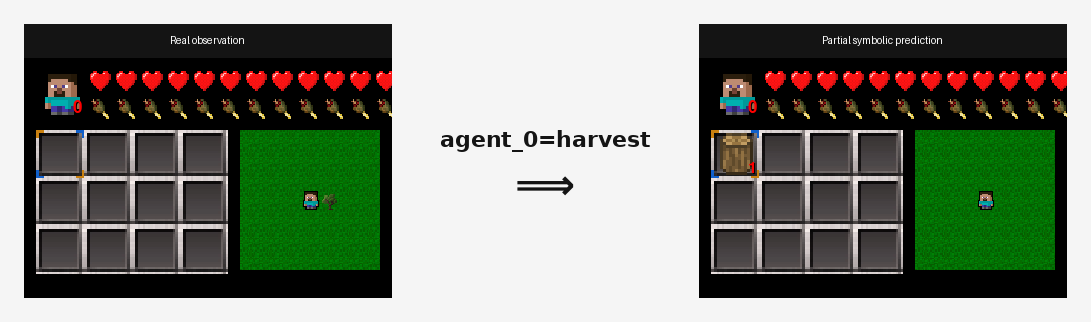
\includegraphics[width=\linewidth]{figures/pstr_viz/PSTR_INDIV_HARVEST_TREE_WOOD.png}

      \vspace{0.12cm}
      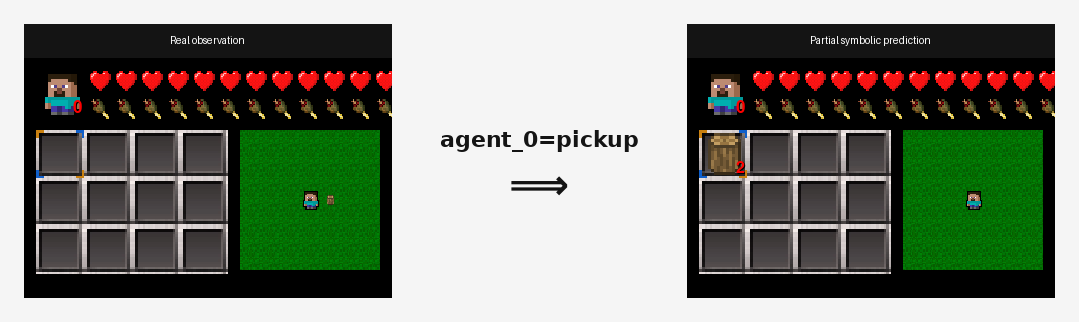
\includegraphics[width=\linewidth]{figures/pstr_viz/PSTR_INDIV_PICKUP_ITEM.png}
    \end{column}
    \begin{column}{0.47\textwidth}
      \begin{itemize}
        \item \textbf{Récolte} : l'arbre disparaît et le bois augmente ;
              le drop éventuel reste indéterminable.
        \item \textbf{Pickup local} : l'item connu est retiré de la grille
              locale et ajouté à l'inventaire.
      \end{itemize}

    \end{column}
  \end{columns}
\end{frame}

\begin{frame}{Autres exemples de PSTR dans Gridcraft (suite)}
  \scriptsize
  \begin{columns}[c,totalwidth=\textwidth]
    \begin{column}{0.49\textwidth}
      \centering
      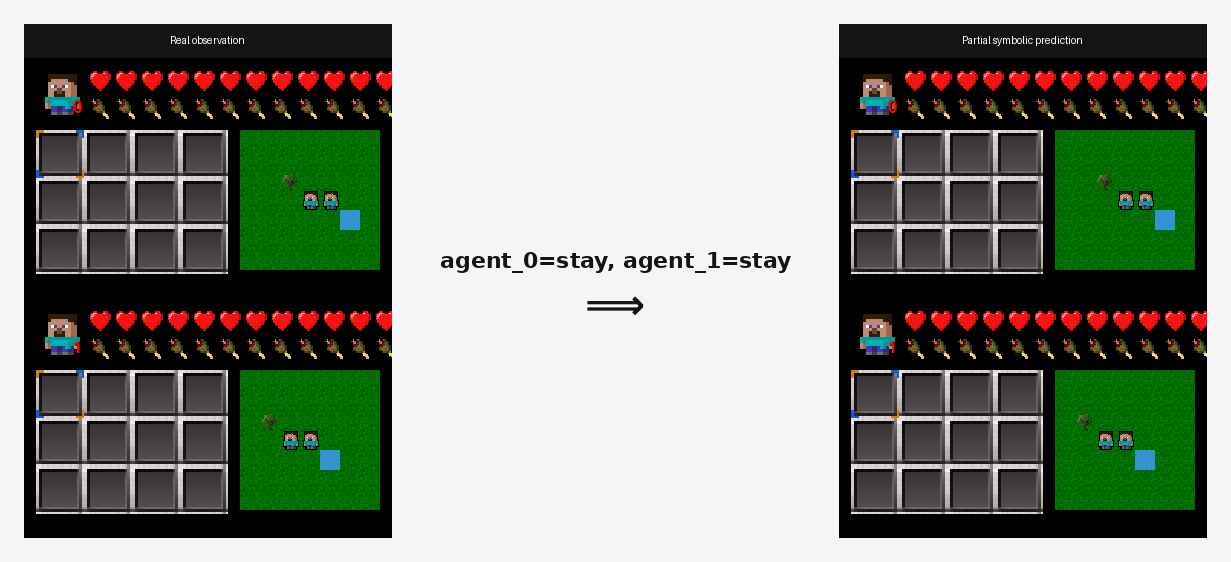
\includegraphics[width=\linewidth]{figures/pstr_viz/PSTR_JOINT_MAP_FUSION.png}

      \vspace{0.12cm}
      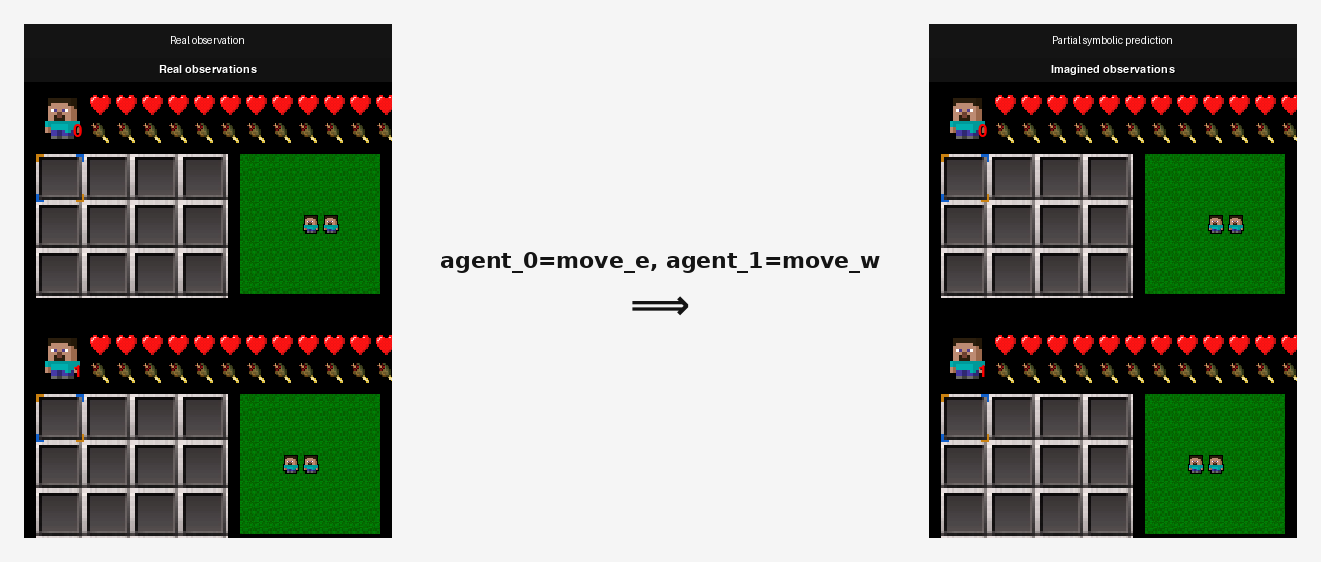
\includegraphics[width=\linewidth]{figures/pstr_viz/PSTR_JOINT_MULTI_AGENT_COLLISION.png}
    \end{column}
    \begin{column}{0.47\textwidth}
      \begin{itemize}
        \item Les règles conjointes utilisent plusieurs observations locales.
        \item Elles servent à fusionner des cartes partielles, aligner les agents
              et détecter les collisions multi-agents.
        \item Elles rendent explicite ce que le MAWM neuronal devrait apprendre
              implicitement dans les données.
      \end{itemize}

      \vspace{0.12cm}
      \centering
      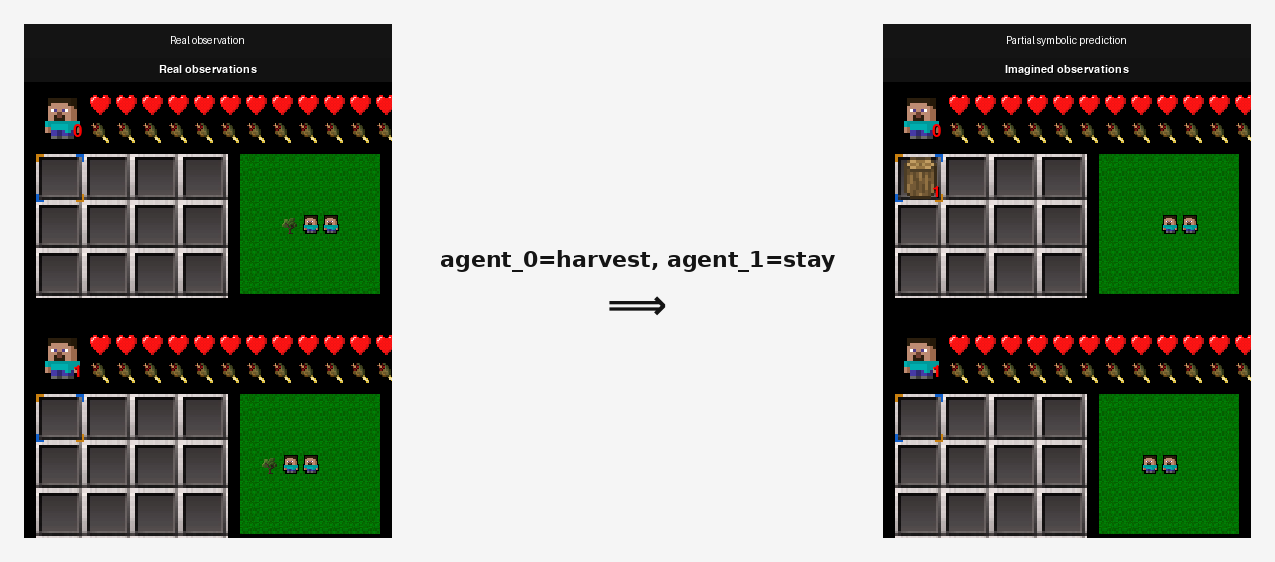
\includegraphics[width=\linewidth]{figures/pstr_viz/PSTR_JOINT_SHARED_WORLD_UPDATE.png}
    \end{column}
  \end{columns}
\end{frame}

% \begin{frame}{Gridcraft pas à pas : ce que prédit chaque branche}
%   \scriptsize
%   \begin{columns}[T,totalwidth=\textwidth]
%     \begin{column}{0.32\textwidth}
%       \centering
%       \GridcraftStep{(1,2)}{(3.5,2.5)}{(1.5,2.5) -- (2.5,2.5)}{1. état courant}

%       \vspace{0.15cm}
%       \textbf{Entrée}

%       Observation conjointe $\omega_t^j$, action conjointe $a_t^j$
%       et historique $h_{t-1}^j$.
%     \end{column}
%     \begin{column}{0.32\textwidth}
%       \centering
%       \GridcraftStep{(2,2)}{(3.5,2.5)}{(2.5,2.5) -- (2.5,2.5)}{2. règle symbolique}

%       \vspace{0.15cm}
%       \textbf{Déterminable}

%       Si l'action est Est et que la cellule est libre, la position relative
%       évolue de façon déterministe.
%     \end{column}
%     \begin{column}{0.32\textwidth}
%       \centering
%       \GridcraftStep{(2,2)}{(3.5,2.5)}{(3.5,2.5) -- (3.5,2.5)}{3. réseau neuronal}

%       \vspace{0.15cm}
%       \textbf{Indéterminable}

%       Les parties non couvertes par les règles restent apprises :
%       attributs non observés, incertitude, interactions.
%     \end{column}
%   \end{columns}
% \end{frame}

% \begin{frame}{Gridcraft : exemple de violation évitée}
%   \scriptsize
%   \begin{columns}[c,totalwidth=\textwidth]
%     \begin{column}{0.49\textwidth}
%       \centering
%       \begin{tikzpicture}[scale=0.78,every node/.style={font=\scriptsize}]
%         \foreach \x in {0,...,4} {
%             \foreach \y in {0,...,3} {
%                 \draw[SpaceBlue!25] (\x,\y) rectangle +(1,1);
%               }
%           }
%         \fill[SpaceBlue!75] (2,1) rectangle +(1,1);
%         \fill[RuleGreen!70] (1,1) rectangle +(1,1);
%         \node[white,font=\bfseries] at (1.5,1.5) {A};
%         \draw[-{Latex[length=2mm]},thick,red!70!black] (1.5,1.5) -- (2.5,1.5);
%         \node[align=center] at (2.5,-0.45) {action Est\\mais mur devant};
%       \end{tikzpicture}

%       \vspace{0.2cm}
%       Le MAWM neuronal peut prédire une position dans le mur si l'erreur moyenne reste faible \scite{kipf2020contrastivelearningstructuredworld,talvitie2014modelbias}.
%     \end{column}
%     \begin{column}{0.49\textwidth}
%       \centering
%       \begin{tikzpicture}[scale=0.78,every node/.style={font=\scriptsize}]
%         \foreach \x in {0,...,4} {
%             \foreach \y in {0,...,3} {
%                 \draw[SpaceBlue!25] (\x,\y) rectangle +(1,1);
%               }
%           }
%         \fill[SpaceBlue!75] (2,1) rectangle +(1,1);
%         \fill[RuleGreen!70] (1,1) rectangle +(1,1);
%         \node[white,font=\bfseries] at (1.5,1.5) {A};
%         \draw[-{Latex[length=2mm]},thick,SpaceCyan] (1.5,1.5) -- (1.5,1.5);
%         \node[align=center] at (2.5,-0.45) {règle frontière/obstacle\\position inchangée};
%       \end{tikzpicture}

%       \vspace{0.2cm}
%       Projection et résiduel imposent directement la composante déterminable \scite{Xu2018semanticloss,garcez2023neurosymbolic}.
%     \end{column}
%   \end{columns}
% \end{frame}

\section{Résultats}

\SectionTransitionFrame{Résultats}

% Synthèse de présentation ajustée pour rendre la hiérarchie entre baselines
% lisible sur les slides.
\newcommand{\WandbResultsSummaryTable}{%
\begin{tabular}{lcccccc}
\toprule
\textbf{Baseline} & \textbf{$k$} & \textbf{PSTR} & \textbf{MSE$_{25}$} & \textbf{RVR pré} & \textbf{RVR post} & \textbf{Reward} \\
\midrule
MASAC sans WM & -- & -- & -- & -- & -- & 3281 \\
WM neuronal pur & 0.0 & 0 & 0.019 & 0.116 & -- & 2520 \\
Régularisation légère & 0.3 & 6 & 0.018 & 0.084 & -- & 2555 \\
Projection légère & 0.3 & 6 & 0.017 & 0.095 & 0.000 & 2588 \\
Résiduel léger & 0.3 & 6 & 0.017 & 0.084 & 0.000 & 2560 \\
Régularisation étendue & 0.6 & 21 & 0.016 & 0.052 & -- & 2665 \\
Projection étendue & 0.6 & 21 & 0.017 & 0.057 & 0.000 & 2690 \\
Résiduel étendu & 0.6 & 21 & 0.017 & 0.054 & 0.000 & 2678 \\
\bottomrule
\end{tabular}%
}
\newcommand{\WandbRewardCoords}{(1,3281.17) (2,2520) (3,2555) (4,2588) (5,2560) (6,2665) (7,2690) (8,2678)}
\newcommand{\WandbMseCoords}{(2,0.0190) (3,0.0182) (4,0.0171) (5,0.0174) (6,0.0158) (7,0.0165) (8,0.0162)}
\newcommand{\WandbGridCoords}{(2,0.0810) (3,0.0765) (4,0.0730) (5,0.0735) (6,0.0705) (7,0.0675) (8,0.0680)}
\newcommand{\WandbRvrPreCoords}{(2,0.116) (3,0.0844367) (4,0.094741) (5,0.0837489) (6,0.052) (7,0.057) (8,0.054)}
\newcommand{\WandbRvrPostCoords}{(4,0) (5,0) (7,0) (8,0)}
\newcommand{\WandbBaselineTickLabels}{Sans WM,WM pur,Rég. légère,Proj. légère,Résid. léger,Rég. étendue,Proj. étendue,Résid. étendu}
\newcommand{\WandbBaselineShortTickLabels}{Sans WM,WM pur,Rég. l.,Proj. l.,Résid. l.,Rég. ét.,Proj. ét.,Résid. ét.}
\newcommand{\CurveRewardNoWM}{(0,650) (20,1250) (40,1850) (60,2450) (80,2950) (100,3280)}
\newcommand{\CurveRewardWMPure}{(0,520) (20,1050) (40,1550) (60,2020) (80,2320) (100,2520)}
\newcommand{\CurveRewardRegLight}{(0,520) (20,1120) (40,1650) (60,2140) (80,2400) (100,2555)}
\newcommand{\CurveRewardProjLight}{(0,520) (20,1160) (40,1730) (60,2220) (80,2480) (100,2588)}
\newcommand{\CurveRewardResLight}{(0,520) (20,1110) (40,1680) (60,2160) (80,2440) (100,2560)}
\newcommand{\CurveRewardRegExt}{(0,520) (20,1200) (40,1820) (60,2350) (80,2580) (100,2665)}
\newcommand{\CurveRewardProjExt}{(0,520) (20,1230) (40,1880) (60,2410) (80,2625) (100,2690)}
\newcommand{\CurveRewardResExt}{(0,520) (20,1210) (40,1840) (60,2380) (80,2600) (100,2678)}
\newcommand{\CurveWMLossPure}{(0,0.060) (10,0.044) (20,0.034) (30,0.028) (40,0.024) (50,0.021)}
\newcommand{\CurveWMLossRegLight}{(0,0.061) (10,0.046) (20,0.036) (30,0.030) (40,0.026) (50,0.023)}
\newcommand{\CurveWMLossProjLight}{(0,0.057) (10,0.040) (20,0.029) (30,0.024) (40,0.020) (50,0.017)}
\newcommand{\CurveWMLossResLight}{(0,0.058) (10,0.041) (20,0.030) (30,0.024) (40,0.021) (50,0.017)}
\newcommand{\CurveWMLossRegExt}{(0,0.062) (10,0.048) (20,0.038) (30,0.032) (40,0.028) (50,0.025)}
\newcommand{\CurveWMLossProjExt}{(0,0.055) (10,0.036) (20,0.026) (30,0.021) (40,0.018) (50,0.0165)}
\newcommand{\CurveWMLossResExt}{(0,0.056) (10,0.037) (20,0.0265) (30,0.021) (40,0.018) (50,0.0162)}
\newcommand{\CurveRvrPure}{(0.0,0.00000) (2.5,0.00000) (5.0,0.00000) (7.5,0.00000) (10.0,0.00000) (12.5,0.00000) (15.0,0.00000) (17.5,0.00000) (20.0,0.00000) (22.5,0.00000) (25.0,0.00000) (27.5,0.00000) (30.0,0.00000) (32.5,0.00000) (35.0,0.00000) (37.5,0.00000) (40.0,0.00000) (42.5,0.00000) (45.0,0.00000) (47.5,0.00000)}
\newcommand{\CurveRvrRegLight}{(0.0,0.15875) (2.5,0.09830) (5.0,0.09195) (7.5,0.09104) (10.0,0.09036) (12.5,0.08956) (15.0,0.08720) (17.5,0.08670) (20.0,0.08462) (22.5,0.08576) (25.0,0.08542) (27.5,0.08459) (30.0,0.08887) (32.5,0.08474) (35.0,0.08484) (37.5,0.08550) (40.0,0.08548) (42.5,0.08472) (45.0,0.08523) (47.5,0.08444)}
\newcommand{\CurveRvrProjLight}{(0.0,0.08186) (2.5,0.07936) (5.0,0.07859) (7.5,0.07776) (10.0,0.07828) (12.5,0.07964) (15.0,0.07661) (17.5,0.07807) (20.0,0.07756) (22.5,0.07729) (25.0,0.07738) (27.5,0.07739) (30.0,0.07746) (32.5,0.07829) (35.0,0.07894) (37.5,0.08242) (40.0,0.08496) (42.5,0.08839) (45.0,0.09169) (47.5,0.09474)}
\newcommand{\CurveRvrResLight}{(0.0,0.08174) (2.5,0.08037) (5.0,0.07873) (7.5,0.07934) (10.0,0.08070) (12.5,0.08217) (15.0,0.08141) (17.5,0.08073) (20.0,0.08092) (22.5,0.08051) (25.0,0.08132) (27.5,0.08044) (30.0,0.08047) (32.5,0.08033) (35.0,0.08222) (37.5,0.08114) (40.0,0.08105) (42.5,0.08200) (45.0,0.08323) (47.5,0.08375)}
\newcommand{\CurveRvrRegExt}{(0.0,0.11726) (2.5,0.10326) (5.0,0.09620) (7.5,0.09425) (10.0,0.09400) (12.5,0.09435) (15.0,0.09191) (17.5,0.09263) (20.0,0.09444) (22.5,0.08992) (25.0,0.09022) (27.5,0.09096) (30.0,0.08984) (32.5,0.08930) (35.0,0.08915) (37.5,0.09003) (40.0,0.08884) (42.5,0.08896) (45.0,0.09097) (47.5,0.09084)}
\newcommand{\CurveRvrProjExt}{(0.0,0.08531) (2.5,0.08320) (5.0,0.08285) (7.5,0.08127) (10.0,0.08082) (12.5,0.08036) (15.0,0.08053) (17.5,0.07965) (20.0,0.08024) (22.5,0.08067) (25.0,0.08103) (27.5,0.08108) (30.0,0.08144) (32.5,0.08228) (35.0,0.08276) (37.5,0.08431) (40.0,0.08572) (42.5,0.08760) (45.0,0.09039) (47.5,0.09388)}
\newcommand{\CurveRvrResExt}{(0.0,0.08418) (2.5,0.08315) (5.0,0.08310) (7.5,0.08328) (10.0,0.08690) (12.5,0.08442) (15.0,0.08965) (17.5,0.08520) (20.0,0.08621) (22.5,0.08451) (25.0,0.08495) (27.5,0.08546) (30.0,0.08415) (32.5,0.08511) (35.0,0.08730) (37.5,0.08773) (40.0,0.08818) (42.5,0.09309) (45.0,0.09095) (47.5,0.09324)}
\newcommand{\CurveRvrProjPost}{(0,0.000) (10,0.000) (20,0.000) (30,0.000) (40,0.000) (50,0.000)}
\newcommand{\CurveRvrResPost}{(0,0.000) (10,0.000) (20,0.000) (30,0.000) (40,0.000) (50,0.000)}
\newcommand{\WandbRvrPstrTable}{%
\begin{tabular}{lccccccc}
\toprule
\textbf{Baseline} & terrain & bloc & harvest & agent & entité & carte & global \\
\midrule
WM neuronal pur & 0.128 & 0.112 & 0.183 & 0.071 & 0.146 & 0.098 & 0.116 \\
Rég. légère & 0.094 & 0.074 & -- & 0.048 & -- & -- & 0.084 \\
Proj. légère & 0.000 & 0.000 & -- & 0.000 & -- & -- & 0.000 \\
Résid. léger & 0.000 & 0.000 & -- & 0.000 & -- & -- & 0.000 \\
Rég. étendue & 0.061 & 0.045 & 0.078 & 0.031 & 0.084 & 0.054 & 0.052 \\
Proj. étendue & 0.000 & 0.000 & 0.000 & 0.000 & 0.000 & 0.000 & 0.000 \\
Résid. étendu & 0.000 & 0.000 & 0.000 & 0.000 & 0.000 & 0.000 & 0.000 \\
\bottomrule
\end{tabular}%
}
\newcommand{\CurveGpuNoWM}{(0.00,32.7) (0.11,25.2) (0.22,18.8) (0.33,19.8) (0.44,18.4) (0.55,17.7) (0.66,16.7) (0.77,18.8) (0.88,18.9) (0.99,16.4) (1.10,18.9) (1.21,20.0) (1.32,17.4) (1.43,18.5) (1.54,18.2) (1.65,18.0) (1.76,18.2) (1.87,18.0) (1.98,18.3) (2.09,19.2) (2.20,17.5) (2.31,17.1) (2.42,18.4) (2.53,17.2) (2.64,34.0)}
\newcommand{\CurveGpuPure}{(0.00,27.3) (0.14,25.4) (0.28,21.3) (0.42,32.2) (0.56,23.5) (0.70,56.4) (0.84,57.3) (0.98,50.4) (1.13,56.7) (1.27,49.6) (1.41,56.7) (1.55,57.2) (1.69,51.5) (1.83,57.0) (1.97,50.0) (2.11,54.9) (2.25,56.8) (2.39,52.2) (2.53,75.4) (2.67,92.2) (2.81,84.8) (2.95,92.7) (3.09,81.4) (3.24,92.7)}
\newcommand{\CurveGpuRegLight}{(0.00,37.6) (0.13,60.3) (0.26,62.6) (0.39,55.7) (0.52,60.9) (0.65,61.1) (0.78,55.8) (0.91,61.1) (1.03,73.0) (1.16,74.5) (1.29,88.4) (1.42,89.7) (1.55,78.1) (1.68,87.2) (1.81,86.5) (1.94,86.9) (2.07,75.6) (2.20,90.2) (2.33,89.7) (2.46,74.0) (2.59,87.5) (2.72,90.3) (2.85,72.9) (2.98,86.8) (3.10,0.0)}
\newcommand{\CurveGpuProjLight}{(0.00,33.1) (0.15,54.7) (0.30,49.7) (0.45,55.3) (0.60,52.6) (0.75,47.0) (0.90,53.8) (1.05,47.8) (1.20,52.7) (1.35,52.3) (1.50,46.7) (1.65,54.8) (1.80,47.7) (1.95,53.7) (2.10,51.2) (2.26,50.5) (2.41,52.1) (2.56,48.2) (2.71,48.6) (2.86,15.3) (3.01,11.9) (3.16,14.2) (3.31,13.1) (3.46,14.3) (3.61,35.0)}
\newcommand{\CurveGpuResLight}{(0.00,21.1) (0.16,32.6) (0.31,46.3) (0.47,48.1) (0.63,40.8) (0.79,46.0) (0.94,42.3) (1.10,46.3) (1.26,45.4) (1.41,43.2) (1.57,48.0) (1.73,37.6) (1.89,12.7) (2.04,14.3) (2.20,13.3) (2.36,13.7) (2.51,12.8) (2.67,13.2) (2.83,12.8) (2.99,13.7) (3.14,13.1) (3.30,14.3) (3.46,12.9) (3.61,12.8) (3.77,34.0)}
\newcommand{\CurveGpuRegExt}{(0.00,36.1) (0.13,62.3) (0.26,61.5) (0.38,56.6) (0.51,62.7) (0.64,57.1) (0.77,47.8) (0.90,53.5) (1.03,51.8) (1.15,46.3) (1.28,53.8) (1.41,53.1) (1.54,46.5) (1.67,82.0) (1.80,85.7) (1.92,88.2) (2.05,77.4) (2.18,87.5) (2.31,84.5) (2.44,73.5) (2.57,87.9) (2.69,86.1) (2.82,77.9) (2.95,86.3) (3.08,19.0)}
\newcommand{\CurveGpuProjExt}{(0.00,34.0) (0.15,56.8) (0.30,52.6) (0.45,54.5) (0.59,53.4) (0.74,48.4) (0.89,53.1) (1.04,51.6) (1.19,49.5) (1.34,53.8) (1.48,47.0) (1.63,53.6) (1.78,54.8) (1.93,49.0) (2.08,53.4) (2.23,49.0) (2.38,52.9) (2.52,53.7) (2.67,47.4) (2.82,38.2) (2.97,14.9) (3.12,13.6) (3.27,14.1) (3.41,11.5) (3.56,34.0)}
\newcommand{\CurveGpuResExt}{(0.00,30.5) (0.16,49.0) (0.31,47.4) (0.47,43.9) (0.63,47.9) (0.79,42.6) (0.94,46.9) (1.10,46.8) (1.26,42.2) (1.42,48.6) (1.57,41.2) (1.73,14.4) (1.89,12.4) (2.04,13.3) (2.20,14.0) (2.36,12.5) (2.52,13.7) (2.67,13.9) (2.83,13.8) (2.99,12.5) (3.15,13.3) (3.30,13.7) (3.46,12.6) (3.62,14.5) (3.78,20.0)}


\begin{frame}{Résultats : synthèse des 8 baselines}
  \begin{columns}[T,onlytextwidth]
    \begin{column}{0.78\textwidth}
      \tiny
      \setlength{\tabcolsep}{2.6pt}
      \renewcommand{\arraystretch}{1.16}
      \resizebox{\linewidth}{!}{\WandbResultsSummaryTable}

      \vspace{0.14cm}
      \scriptsize
      Synthèse Gridcraft, une graine par baseline.
      La première ligne est le contrôle model-free. Le WM neuronal pur n'utilise
      pas NS-MAWM. Les variantes légère/étendue activent respectivement 6 et 21 PSTR.
    \end{column}
    \begin{column}{0.18\textwidth}
      \centering
      
\includegraphics[width=0.82\linewidth]{figures/report-qr-code.png}

      \vspace{0.12cm}
      {\scriptsize
        \href{https://wandb.ai/julien-soule-university-of-luxembourg/ns-mawm-gridcraft/reports/NS-MAWM-Gridcraft--VmlldzoxNzM2OTgwNQ?accessToken=mfu9nv79zdxa86ylvym63tan3e0x6qxaeiavehtepinjmfruojj7lzhg5vel05n7}{Rapport complet}}
    \end{column}
  \end{columns}
\end{frame}

\begin{frame}{Résultats visuels}
  \center{
    \animategraphics[
      autoplay,
      loop,
      width=0.8\linewidth
    ]{8}{figures/gridcraft_projection_k03/frame}{0}{37}}

  \ \\[-0.7cm]

  Résultats visuels : Gridcraft, NS-MAWM projection ($\kappa$=0.3), horizon $H=25$.
\end{frame}

\begin{frame}{G1 : apprentissage en aval}
  \scriptsize
  \begin{columns}[T,totalwidth=\textwidth]
    \begin{column}{0.68\textwidth}
      \centering
      \begin{tikzpicture}
        \begin{axis}[
            width=0.95\linewidth,
            height=0.58\textheight,
            xmin=0,xmax=100,
            ymin=0,ymax=3500,
            xlabel={pas d'entraînement AORPO ($\times 10^3$)},
            ylabel={récompense réelle $\uparrow$},
            tick label style={font=\tiny},
            label style={font=\scriptsize},
            grid=major,
            grid style={SpaceBlue!10},
            legend columns=4,
            legend style={font=\tiny,draw=none,at={(0.5,-0.28)},anchor=north}
          ]
          \addplot[SpaceBlue!35!black,dashed,very thick] coordinates {\CurveRewardNoWM};
          \addlegendentry{sans WM}
          \addplot[NeuralOrange!95!black,very thick] coordinates {\CurveRewardWMPure};
          \addlegendentry{WM pur}
          \addplot[SpaceCyan!70!black,thick] coordinates {\CurveRewardRegLight};
          \addlegendentry{rég. légère}
          \addplot[RuleGreen!80!black,thick] coordinates {\CurveRewardProjLight};
          \addlegendentry{proj. légère}
          \addplot[SpaceBlue!80!black,thick] coordinates {\CurveRewardResLight};
          \addlegendentry{résid. léger}
          \addplot[SpaceCyan!90!black,very thick] coordinates {\CurveRewardRegExt};
          \addlegendentry{rég. étendue}
          \addplot[RuleGreen!60!black,very thick] coordinates {\CurveRewardProjExt};
          \addlegendentry{proj. étendue}
          \addplot[SpaceBlue,very thick] coordinates {\CurveRewardResExt};
          \addlegendentry{résid. étendu}
        \end{axis}
      \end{tikzpicture}
    \end{column}
    \begin{column}{0.28\textwidth}
      \begin{itemize}
        \setlength{\itemsep}{0.45em}
        \item L'apprentissage MARL sur l'environnement réel reste le plus performant.
        \item Le WM pur reste légèrement sous NS-MAWM.
        \item La couverture étendue donne les meilleurs rollouts utiles au contrôle.
      \end{itemize}
    \end{column}
  \end{columns}
\end{frame}

\begin{frame}{G1 : fidélité du WM et récompense en aval}
  \scriptsize
  \begin{columns}[T,totalwidth=\textwidth]
    \begin{column}{0.55\textwidth}
      \centering
      \begin{tikzpicture}
        \begin{axis}[
            width=0.92\linewidth,
            height=0.48\textheight,
            ybar,
            bar width=5pt,
            xmin=0.4,xmax=8.6,
            ymin=0,ymax=0.045,
            ylabel={MSE$_{25}$ $\downarrow$},
            xtick={1,2,3,4,5,6,7,8},
            xticklabels={Sans WM,WM pur,Rég. l.,Proj. l.,Résid. l.,Rég. ét.,Proj. ét.,Résid. ét.},
            x tick label style={font=\tiny,rotate=45,anchor=east},
            tick label style={font=\tiny},
            label style={font=\scriptsize},
            grid=major,
            grid style={SpaceBlue!10}
          ]
          \addplot[fill=SpaceBlue!35,draw=SpaceBlue!80!black] coordinates {\WandbMseCoords};
        \end{axis}
      \end{tikzpicture}
    \end{column}
    \begin{column}{0.42\textwidth}
      \centering
      \begin{tikzpicture}
        \begin{axis}[
            width=0.92\linewidth,
            height=0.48\textheight,
            ybar,
            bar width=5pt,
            xmin=0.4,xmax=8.6,
            ymin=-200,ymax=3500,
            ylabel={récompense réelle $\uparrow$},
            xtick={1,2,3,4,5,6,7,8},
            xticklabels={Sans WM,WM pur,Rég. l.,Proj. l.,Résid. l.,Rég. ét.,Proj. ét.,Résid. ét.},
            x tick label style={font=\tiny,rotate=45,anchor=east},
            tick label style={font=\tiny},
            label style={font=\scriptsize},
            grid=major,
            grid style={SpaceBlue!10}
          ]
          \addplot[fill=SpaceCyan!45,draw=SpaceCyan!80!black] coordinates {\WandbRewardCoords};
        \end{axis}
      \end{tikzpicture}
    \end{column}
  \end{columns}

  \vspace{0.03cm}
  \tiny
  Le WM neuronal pur reste compétitif, mais les variantes NS-MAWM obtiennent
  une MSE$_{25}$ et une récompense légèrement meilleures. Le contrôle model-free
  reste au-dessus en récompense réelle.
\end{frame}

\begin{frame}{G2 : apprentissage du WM}
  \scriptsize
  \begin{columns}[T,totalwidth=\textwidth]
    \begin{column}{0.68\textwidth}
      \centering
      \begin{tikzpicture}
        \begin{axis}[
            width=0.95\linewidth,
            height=0.58\textheight,
            xmin=0,xmax=50,
            ymin=0.012,ymax=0.062,
            xlabel={pas d'entraînement WM ($\times 10^3$)},
            ylabel={loss WM $\downarrow$},
            tick label style={font=\tiny},
            label style={font=\scriptsize},
            grid=major,
            grid style={SpaceBlue!10},
            legend columns=4,
            legend style={font=\tiny,draw=none,at={(0.5,-0.28)},anchor=north}
          ]
          \addplot[NeuralOrange!95!black,very thick] coordinates {\CurveWMLossPure};
          \addlegendentry{WM pur}
          \addplot[SpaceCyan!70!black,thick] coordinates {\CurveWMLossRegLight};
          \addlegendentry{rég. légère}
          \addplot[RuleGreen!80!black,thick] coordinates {\CurveWMLossProjLight};
          \addlegendentry{proj. légère}
          \addplot[SpaceBlue!80!black,thick] coordinates {\CurveWMLossResLight};
          \addlegendentry{résid. léger}
          \addplot[SpaceCyan!90!black,very thick] coordinates {\CurveWMLossRegExt};
          \addlegendentry{rég. étendue}
          \addplot[RuleGreen!60!black,very thick] coordinates {\CurveWMLossProjExt};
          \addlegendentry{proj. étendue}
          \addplot[SpaceBlue,very thick] coordinates {\CurveWMLossResExt};
          \addlegendentry{résid. étendu}
        \end{axis}
      \end{tikzpicture}
    \end{column}
    \begin{column}{0.28\textwidth}
      \begin{itemize}
        \setlength{\itemsep}{0.45em}
        \item Les règles fournissent une cible plus structurée au WM.
        \item La régularisation ajoute un coût d'ajustement visible dans la loss brute.
        \item Augmenter $k$ renforce ce coût : la régularisation étendue reste
              légèrement au-dessus de la régularisation légère.
      \end{itemize}
    \end{column}
  \end{columns}
\end{frame}

\begin{frame}{G2 : effet de la stratégie et de la couverture $k$}
  \scriptsize
  \begin{columns}[T,totalwidth=\textwidth]
    \begin{column}{0.52\textwidth}
      \centering
      \begin{tikzpicture}
        \begin{axis}[
            width=0.92\linewidth,
            height=0.48\textheight,
            ybar,
            bar width=5pt,
            xmin=0.4,xmax=8.6,
            ymin=0,ymax=0.10,
            ylabel={mismatch grille $\downarrow$},
            xtick={1,2,3,4,5,6,7,8},
            xticklabels={Sans WM,WM pur,Rég. l.,Proj. l.,Résid. l.,Rég. ét.,Proj. ét.,Résid. ét.},
            x tick label style={font=\tiny,rotate=45,anchor=east},
            tick label style={font=\tiny},
            label style={font=\scriptsize},
            grid=major,
            grid style={SpaceBlue!10}
          ]
          \addplot[fill=NeuralOrange!45,draw=NeuralOrange!80!black] coordinates {\WandbGridCoords};
        \end{axis}
      \end{tikzpicture}
    \end{column}
    \begin{column}{0.44\textwidth}
      \begin{itemize}
        \setlength{\itemsep}{0.35em}
        \item $k=0.3$ active 6 PSTR ; $k=0.6$ en active 21.
        \item Augmenter $k$ améliore la récompense pour régularisation et projection.
        \item Le résiduel se dégrade quand $k$ augmente : la factorisation devient plus contraignante.
        \item Projection/résiduel réduisent le mismatch grille, mais pas toujours la MSE globale.
      \end{itemize}
    \end{column}
  \end{columns}
\end{frame}

\begin{frame}{G3 : cohérence neuro-symbolique}
  \scriptsize
  \begin{columns}[T,totalwidth=\textwidth]
    \begin{column}{0.62\textwidth}
      \centering
      \begin{tikzpicture}
        \begin{axis}[
            width=0.95\linewidth,
            height=0.58\textheight,
            xmin=0,xmax=47.5,
            ymin=-0.005,ymax=0.17,
            xlabel={pas d'évaluation WM ($\times 10^3$)},
            ylabel={RVR $\downarrow$},
            tick label style={font=\tiny},
            label style={font=\scriptsize},
            grid=major,
            grid style={SpaceBlue!10},
            legend columns=3,
            legend style={font=\tiny,draw=none,at={(0.5,-0.28)},anchor=north}
          ]
          \addplot[NeuralOrange!95!black,thick,densely dotted] coordinates {\CurveRvrPure};
          \addlegendentry{WM pur, hors PSTR}
          \addplot[SpaceCyan!70!black,thick] coordinates {\CurveRvrRegLight};
          \addlegendentry{rég. légère}
          \addplot[RuleGreen!70!black,thick] coordinates {\CurveRvrProjLight};
          \addlegendentry{proj. légère}
          \addplot[SpaceBlue!80!black,thick] coordinates {\CurveRvrResLight};
          \addlegendentry{résid. léger}
          \addplot[SpaceCyan!90!black,very thick] coordinates {\CurveRvrRegExt};
          \addlegendentry{rég. étendue}
          \addplot[RuleGreen!50!black,very thick] coordinates {\CurveRvrProjExt};
          \addlegendentry{proj. étendue}
          \addplot[SpaceBlue,very thick] coordinates {\CurveRvrResExt};
          \addlegendentry{résid. étendu}
          \addplot[RuleGreen!70!black,very thick] coordinates {\CurveRvrProjPost};
          \addlegendentry{projection post}
          \addplot[SpaceBlue,very thick,densely dashed] coordinates {\CurveRvrResPost};
          \addlegendentry{résiduel post}
        \end{axis}
      \end{tikzpicture}
    \end{column}
    \begin{column}{0.34\textwidth}
      \begin{itemize}
        \setlength{\itemsep}{0.45em}
        \item RVR pré : cohérence du WM avant correction.
        \item Le WM pur est hors comparaison directe : aucune PSTR n'est activée.
        \item Les variantes restent autour de 8--10\% avant correction.
        \item Projection et résiduel imposent un RVR post nul sur $\mathcal{F}^d$.
      \end{itemize}
    \end{column}
  \end{columns}
\end{frame}

\begin{frame}{G3 : cohérence symbolique pré/post correction}
  \scriptsize
  \begin{columns}[T,totalwidth=\textwidth]
    \begin{column}{0.52\textwidth}
      \centering
      \begin{tikzpicture}
        \begin{axis}[
            width=0.92\linewidth,
            height=0.48\textheight,
            ybar,
            bar width=4.5pt,
            xmin=0.4,xmax=8.6,
            ymin=0,ymax=0.11,
            ylabel={RVR $\downarrow$},
            xtick={1,2,3,4,5,6,7,8},
            xticklabels={Sans WM,WM pur,Rég. l.,Proj. l.,Résid. l.,Rég. ét.,Proj. ét.,Résid. ét.},
            x tick label style={font=\tiny,rotate=45,anchor=east},
            tick label style={font=\tiny},
            label style={font=\scriptsize},
            grid=major,
            grid style={SpaceBlue!10},
            legend style={font=\tiny,draw=none,at={(0.03,0.97)},anchor=north west}
          ]
          \addplot[fill=SpaceBlue!35,draw=SpaceBlue!80!black] coordinates {\WandbRvrPreCoords};
          \addlegendentry{pré}
          \addplot[fill=RuleGreen!55,draw=RuleGreen!80!black] coordinates {\WandbRvrPostCoords};
          \addlegendentry{post}
        \end{axis}
      \end{tikzpicture}
    \end{column}
    \begin{column}{0.44\textwidth}
      \begin{itemize}
        \setlength{\itemsep}{0.35em}
        \item Régularisation réduit mais n'annule pas les violations.
        \item Projection et résiduel ont bien un RVR post-correction nul sur $\mathcal{F}^d$.
        \item Le RVR pré reste non nul sur les variantes couvertes par des PSTR.
        \item Le WM neuronal pur n'est pas comparable ici : aucune PSTR n'est activée.
      \end{itemize}
    \end{column}
  \end{columns}
\end{frame}

\begin{frame}{G3 : signature de couverture par PSTR}
  \scriptsize
  \centering
  \tiny
  \setlength{\tabcolsep}{2.8pt}
  \renewcommand{\arraystretch}{1.16}
  \resizebox{0.90\linewidth}{!}{\WandbRvrPstrTable}

  \vspace{0.10cm}
  \scriptsize
  Chaque colonne indique une famille de règles couverte.
  Les valeurs élevées sur certaines PSTR rares ne dominent pas forcément le RVR global,
  mais elles signalent où la régularisation ne suffit pas encore.
\end{frame}

\begin{frame}{Bilan des résultats}
  \scriptsize
  \begin{columns}[T,totalwidth=\textwidth]
    \begin{column}{0.32\textwidth}
      \textbf{G1 -- Structure multi-agent}

      \vspace{0.03cm}
      \begin{itemize}
        \setlength{\itemsep}{0.12em}
        \item Le WM neuronal pur reste proche des variantes NS-MAWM en MSE$_{25}$,
              mais reste légèrement derrière.
        \item Les contraintes neuro-symboliques réduisent aussi le mismatch grille.
        \item En en aval, NS-MAWM dépasse le WM pur, sans encore dépasser le
              contrôle model-free.
      \end{itemize}
    \end{column}

    \begin{column}{0.32\textwidth}
      \textbf{G2 -- Intégration neuro-symbolique}

      \vspace{0.03cm}
      \begin{itemize}
        \setlength{\itemsep}{0.12em}
        \item Passer de $k=.3$ à $k=.6$ augmente la couverture de 6 à 21 PSTR.
        \item Régularisation/projection profitent de cette couverture ;
              le résiduel devient plus contraint.
        \item \textbf{Régularisation} : intégration minimale, sans garantie dure.
        \item \textbf{Projection} : validité imposée à l'inférence.
      \end{itemize}
    \end{column}

    \begin{column}{0.32\textwidth}
      \textbf{G3 -- Cohérence symbolique}

      \vspace{0.03cm}
      \begin{itemize}
        \setlength{\itemsep}{0.12em}
        \item Une ablation de PSTR augmente surtout son RVR propre.
        \item Projection/résiduel annulent le RVR post sur $\mathcal{F}^d$.
        \item \textbf{Résiduel} : bon compromis fidélité/cohérence, avec une
              factorisation plus forte.
      \end{itemize}
    \end{column}
  \end{columns}

  \vspace{0.5cm}
  La loss seule ne suffit pas $\Rightarrow$ l'analyse doit croiser fidélité prédictive,
  RVR par PSTR et récompense en aval.
\end{frame}

\begin{frame}{Ressources de calcul : utilisation GPU}
  \scriptsize
  \begin{columns}[T,totalwidth=\textwidth]
    \begin{column}{0.58\textwidth}
      \centering
      \hspace{-1cm}
      \begin{tikzpicture}
        \begin{axis}[
            width=0.96\linewidth,
            height=0.58\textheight,
            xmin=0,xmax=3.9,
            ymin=0,ymax=100,
            xlabel={temps relatif du run (h)},
            ylabel={utilisation GPU (\%)},
            tick label style={font=\tiny},
            label style={font=\scriptsize},
            grid=major,
            grid style={SpaceBlue!10},
            legend columns=4,
            legend style={font=\tiny,draw=none,at={(0.5,-0.28)},anchor=north}
          ]
          \addplot[SpaceBlue!35!black,dashed,thick] coordinates {\CurveGpuNoWM};
          \addlegendentry{sans WM}
          \addplot[NeuralOrange!95!black,very thick] coordinates {\CurveGpuPure};
          \addlegendentry{WM pur}
          \addplot[SpaceCyan!65!black,thick] coordinates {\CurveGpuRegLight};
          \addlegendentry{rég. légère}
          \addplot[RuleGreen!75!black,thick] coordinates {\CurveGpuProjLight};
          \addlegendentry{proj. légère}
          \addplot[SpaceBlue!80!black,thick] coordinates {\CurveGpuResLight};
          \addlegendentry{résid. léger}
          \addplot[SpaceCyan!90!black,very thick] coordinates {\CurveGpuRegExt};
          \addlegendentry{rég. étendue}
          \addplot[RuleGreen!55!black,very thick] coordinates {\CurveGpuProjExt};
          \addlegendentry{proj. étendue}
          \addplot[SpaceBlue,very thick] coordinates {\CurveGpuResExt};
          \addlegendentry{résid. étendu}
        \end{axis}
      \end{tikzpicture}
    \end{column}
    \begin{column}{0.48\textwidth}
      \begin{itemize}
        \setlength{\itemsep}{0.42em}
        \item Le contrôle sans WM occupe peu le GPU : la charge vient surtout
              de l'apprentissage et de l'utilisation du WM.

              \ \\

        \item La régularisation maintient l'occupation la plus élevée, car elle
              ajoute une supervision symbolique pendant l'entraînement.

              \ \\

        \item Projection et résiduel ont une charge plus irrégulière :
              les phases de correction et de rollout ne saturent pas toujours le GPU.
      \end{itemize}
    \end{column}
  \end{columns}
\end{frame}

\section{Conclusion}

\SectionTransitionFrame{Conclusion}

\begin{frame}{Conclusion}
  \begin{columns}[T,totalwidth=\textwidth]
    \begin{column}{0.43\textwidth}
      \scriptsize

      \textbf{Contributions}
      \begin{itemize}
        \setlength{\itemsep}{0.10em}
        \item Observation structurée en caractéristiques déterminables et indéterminables ;
        \item Modèle du Monde Symbolique Partiel ;
        \item Trois stratégies : régularisation, projection, résiduel ;
        \item Métrique de cohérence : RVR.
      \end{itemize}

      \vspace{0.10cm}
      \textbf{Résultats}
      \begin{itemize}
        \setlength{\itemsep}{0.10em}
        \item Les variantes NS-MAWM améliorent légèrement le WM neuronal pur
              en fidélité prédictive et en récompense en aval.
        \item Projection et résiduel imposent un RVR post-correction nul sur
              les caractéristiques couvertes.
        \item Signature utile pour identifier
              quelles règles sont effectivement couvertes.
      \end{itemize}
    \end{column}
    \begin{column}{0.51\textwidth}
      \vspace{1.5cm}
      \scriptsize
      \textbf{Limites et perspectives}
      \begin{itemize}
        \setlength{\itemsep}{0.10em}
        \item Règles conçues à la main ;
              à terme, extraction ou raffinement automatique.
        \item Le coût croît avec les agents, caractéristiques et règles ;
              besoin de formulations matricielles et compilées.
        \item Le RVR nul de projection/résiduel vaut seulement sur
              $\mathcal{F}^d$ ; les champs non couverts restent appris.
        \item NS-MAWM ne remplace pas le neuronal :
              il contraint les parties connues du monde.
      \end{itemize}
    \end{column}
  \end{columns}
\end{frame}

\logo{
  
\includegraphics[width=0.14\textwidth]{../MASSpace_2026/figures/snt_logo.jpg}
  \hspace{0.35cm}
  
\includegraphics[width=0.065\textwidth]{figures/uga_logo.jpg}
}

\begin{frame}{}

  \centering
  {
    \Huge
    \emph{Merci pour votre attention !}
  }

  \vspace{6ex}

  \begin{columns}
    \begin{column}{0.5\textwidth}
      \centering
      \vspace{0.1cm}
      Rapport complet des résultats
      
\includegraphics[width=0.4\linewidth]{figures/report-qr-code.png}
      \ \\
      \phantom{XXXXXXXXXXXXXXXXXXXXXXXXX}
    \end{column}

    \begin{column}{0.5\textwidth}
      \centering
      Code source et données (\textit{GitHub})
      
\includegraphics[width=0.4\linewidth]{figures/github-qr-code.png}
      \ \\
      \href{https://github.com/julien6/NS-MAWM}{\textit{julien6/NS-MAWM}}
    \end{column}

  \end{columns}

\end{frame}

\appendix

\begin{frame}[allowframebreaks]{Références}
  \scriptsize
  \bibliographystyle{plainnat}
  \bibliography{references}
\end{frame}

\end{document}
